\documentclass[11pt,a4paper]{article}

% --- Encoding & fonts -------------------------------------------------------
\usepackage[utf8]{inputenc}
\usepackage[T1]{fontenc}
\usepackage{lmodern}                 % modern Computer Modern (better screen)
\usepackage{microtype}               % protrusion + expansion (cleaner lines)
\usepackage{amsmath,amssymb,amsfonts}

% --- Page geometry: wider text column for larger figures --------------------
\usepackage[a4paper,
            top=0.95in, bottom=1.0in,
            left=0.85in, right=0.85in,
            footskip=0.45in]{geometry}

% --- Floats, captions, tables -----------------------------------------------
\usepackage{graphicx}
\usepackage{subcaption}
\usepackage{booktabs}
\usepackage[font=small,            % caption text slightly smaller than body
            labelfont=bf,          % bold "Figure 1:" label
            justification=justified,
            singlelinecheck=false,
            skip=6pt,
            margin=8pt]{caption}

% --- Colour & links ---------------------------------------------------------
\usepackage{xcolor}
\usepackage{url}
\usepackage[colorlinks=true,
            linkcolor={blue!55!black},
            citecolor={blue!55!black},
            urlcolor={blue!55!black},
            breaklinks=true]{hyperref}
\usepackage{tcolorbox}

% --- Spacing for readability -----------------------------------------------
\linespread{1.06}                    % a hair more line spacing than default
\setlength{\parskip}{0.45em plus 0.1em minus 0.05em}
\setlength{\parindent}{0pt}          % paragraphs separated by vertical space
\setlength{\abovecaptionskip}{6pt}
\setlength{\belowcaptionskip}{2pt}
\setlength{\textfloatsep}{16pt plus 2pt minus 4pt}
\setlength{\intextsep}{16pt plus 2pt minus 4pt}

% Section headings: a bit more breathing room
\usepackage{titlesec}
\titlespacing*{\section}     {0pt}{2.0ex plus 0.6ex minus 0.4ex}{1.0ex plus 0.3ex}
\titlespacing*{\subsection}  {0pt}{1.6ex plus 0.5ex minus 0.3ex}{0.8ex plus 0.2ex}
\titlespacing*{\subsubsection}{0pt}{1.3ex plus 0.4ex minus 0.3ex}{0.6ex plus 0.2ex}

% Epistemic classification boxes
\newtcolorbox{theorem_box}[1][]{colback=green!5,colframe=green!50!black,title=\textbf{Theorem (Mathematical Consequence)},#1}
\newtcolorbox{assumption_box}[1][]{colback=blue!5,colframe=blue!50!black,title=\textbf{Physically Motivated Assumption},#1}
\newtcolorbox{occam_box}[1][]{colback=orange!5,colframe=orange!50!black,title=\textbf{Minimal Complexity Choice},#1}

\title{Robust Non-Singular Bouncing Cosmology\\from Regularized Hyperbolic Field Space}

\author{Oleksandr Kravchenko}
\date{%
    \small \textit{UponCode LLC, Research Division, Cheyenne, WY, USA}\\%
    \textit{OkMath Research Initiative}\\[2ex]%
    \footnotesize \texttt{cosmology@okmath.org}%
}

\begin{document}

% Fallback values — overwritten by results_macros.tex when present.
% These must stay in sync with the values produced by the current
% run_all_tests.py output; otherwise a build without results_macros.tex
% will silently use stale numbers.
\providecommand{\nsAnalytical}{0.9667}
\providecommand{\rAnalytical}{0.0033}
\providecommand{\AsAnalytical}{2.23e-09}
\providecommand{\constraintMedian}{1.2}
\providecommand{\constraintPninetyfive}{5.3}
\providecommand{\HCmedian}{10^{-4}}
\providecommand{\nsNumerical}{0.9923}
\providecommand{\fitMaxResidual}{0.050}
\providecommand{\nsCMBnumerical}{0.9683}
\providecommand{\nsCMBexactFit}{0.9678}
\providecommand{\nsCMBleading}{0.9667}
\providecommand{\nsCMBdelta}{5.47e-04}
\providecommand{\nsCMBdeltaLeading}{1.67e-03}
\providecommand{\nCMBmodes}{11}
\providecommand{\AsRatioMean}{1.035}
\providecommand{\AsAgreementPct}{3.5}
\providecommand{\nAlphaPoints}{11}
\providecommand{\nsAlphaMean}{0.9672}
\providecommand{\phiCMBmeasured}{5.4290}
\providecommand{\NactualAtCMB}{60.000}
\providecommand{\NtotalInflationAlphaScan}{86.44}
\providecommand{\nAlphaPointsNT}{11}
\providecommand{\nsAlphaMeanNT}{0.96699}
\providecommand{\nsAlphaStdNT}{2.40e-06}
\providecommand{\nsAlphaSpreadNT}{8.25e-06}
\providecommand{\KchiMaxNT}{11.6}
\providecommand{\gCMBminNT}{0.748}
\providecommand{\gCMBmaxNT}{1.000}
\providecommand{\nsFitKgeqFive}{0.99228}
\providecommand{\nsFitKgeqFiveModes}{11}
\providecommand{\nsFitKgeqFiveRes}{0.050}
\providecommand{\nsFitKgeqTen}{0.99741}
\providecommand{\nsFitKgeqTenModes}{9}
\providecommand{\nsFitKgeqTenRes}{0.008}
\providecommand{\nsFitKgeqFifteen}{0.99963}
\providecommand{\nsFitKgeqFifteenModes}{8}
\providecommand{\nsFitKgeqFifteenRes}{0.002}
\providecommand{\nsFitKgeqTwenty}{1.00045}
\providecommand{\nsFitKgeqTwentyModes}{7}
\providecommand{\nsFitKgeqTwentyRes}{0.001}
\providecommand{\bumpAmpLnT}{1.97}
\providecommand{\bumpKpeak}{0.72}
\providecommand{\bumpSigmaLnK}{0.45}
\providecommand{\bumpNtotal}{2630}
\providecommand{\NhiddenEfolds}{2570}
\providecommand{\RConservationDelta}{4.43e-03}
\providecommand{\RConservationNearly}{1.0}
\providecommand{\RConservationNlate}{5.0}
\providecommand{\cSSqMaxDev}{8e-16}
\providecommand{\cTSqMaxDev}{0e+00}
\providecommand{\cSEffDeviation}{0.00e+00}
\providecommand{\turnRateMax}{0.00e+00}
\providecommand{\cSProbeCount}{203}
\providecommand{\NpostBounce}{398.0}
\providecommand{\fNLCMBdeltaN}{+0.0133}
\providecommand{\fNLCMBconsistency}{+0.0134}
\providecommand{\fNLCMBconsistencyLeading}{+0.0139}
\providecommand{\fNLCMBdelta}{1.54e-04}
\providecommand{\fNLCMBdeltaLeading}{6.38e-04}
\providecommand{\fNLBounce}{+3.16e-04}
\providecommand{\logTenkCMBoverkH}{1116}
\providecommand{\logTenfNLBounceAtCMB}{-2232}
\providecommand{\attractorRelErrMedian}{1.4e-04}
\providecommand{\attractorRelErrMax}{1.4e-04}
\providecommand{\attractorPhiRangeLo}{9.836}
\providecommand{\attractorPhiRangeHi}{9.957}
\IfFileExists{results_macros.tex}{% Auto-generated by run_all_tests.py -- do not edit manually
\def\aMinBounce{1.73e+05}
\def\NpostBounce{398.0}
\def\HBounce{-5.22e-09}
\def\gDeviationMax{3.1e-09}
\def\nsAnalytical{0.9667}
\def\rAnalytical{0.0033}
\def\AsAnalytical{2.23e-09}
\def\nAlphaPoints{11}
\def\nsAlphaStd{0.000000}
\def\nsAlphaMean{0.9672}
\def\phiCMBmeasured{5.4290}
\def\NactualAtCMB{60.000}
\def\NtotalInflationAlphaScan{86.44}
\def\nAlphaPointsNT{11}
\def\nsAlphaMeanNT{0.96699}
\def\nsAlphaStdNT{2.40e-06}
\def\nsAlphaSpreadNT{8.25e-06}
\def\KchiMaxNT{11.6}
\def\gCMBminNT{0.748}
\def\gCMBmaxNT{1.000}
\def\nsNumerical{0.9923}
\def\nModesConverged{16}
\def\TRSmax{0.0000e+00}
\def\constraintMedian{1.2}
\def\constraintPninetyfive{5.3}
\def\HCmedian{10^{-4}}
\def\fitMaxResidual{0.050}
\def\nsFitKgeqFive{0.99228}
\def\nsFitKgeqFiveModes{11}
\def\nsFitKgeqFiveRes{0.050}
\def\nsFitKgeqTen{0.99741}
\def\nsFitKgeqTenModes{9}
\def\nsFitKgeqTenRes{0.008}
\def\nsFitKgeqFifteen{0.99963}
\def\nsFitKgeqFifteenModes{8}
\def\nsFitKgeqFifteenRes{0.002}
\def\nsFitKgeqTwenty{1.00045}
\def\nsFitKgeqTwentyModes{7}
\def\nsFitKgeqTwentyRes{0.001}
\def\bumpAmpLnT{1.97}
\def\bumpKpeak{0.72}
\def\bumpSigmaLnK{0.45}
\def\bumpNtotal{2630}
\def\NhiddenEfolds{2570}
\def\nsCMBnumerical{0.9683}
\def\nsCMBexactFit{0.9678}
\def\nsCMBleading{0.9667}
\def\nsCMBdelta{5.47e-04}
\def\nsCMBdeltaLeading{1.67e-03}
\def\nCMBmodes{11}
\def\AsRatioMean{1.035}
\def\AsAgreementPct{3.5}
\def\RConservationDelta{4.43e-03}
\def\RConservationNearly{1.0}
\def\RConservationNlate{5.0}
\def\RConservationK{0.50}
\def\cSSqMaxDev{8e-16}
\def\cTSqMaxDev{0e+00}
\def\cSEffDeviation{0.00e+00}
\def\turnRateMax{0.00e+00}
\def\cSPositivity{yes}
\def\cTPositivity{yes}
\def\cSProbeCount{203}
\def\HAtBounceSample{-5.2e-09}
\def\fNLCMBdeltaN{+0.0133}
\def\fNLCMBconsistency{+0.0134}
\def\fNLCMBconsistencyLeading{+0.0139}
\def\fNLCMBdelta{1.54e-04}
\def\fNLCMBdeltaLeading{6.38e-04}
\def\fNLBounce{+3.16e-04}
\def\logTenkCMBoverkH{1116}
\def\logTenfNLBounceAtCMB{-2232}
\def\attractorRelErrMedian{1.4e-04}
\def\attractorRelErrMax{1.4e-04}
\def\attractorPhiRangeLo{9.836}
\def\attractorPhiRangeHi{9.957}
}{}

\maketitle

\begin{abstract}
We construct a non-singular bouncing cosmology in a closed ($k=+1$) universe with a two-field sigma model whose field-space metric $g_{\chi\chi} = (1 + e^{-2\alpha\phi/M_{\rm Pl}})^{-1}$ is determined by three physical boundary conditions and a minimal-complexity selection principle. The model satisfies the Null Energy Condition, avoids ghosts, and achieves BKL stability within the homogeneous Bianchi~IX truncation, all in standard General Relativity.

We integrate the full two-field perturbation system $(\delta\phi, \delta\chi, \Phi)$ in the Newtonian gauge through the bounce over 65 e-folds, circumventing the gauge singularity of the comoving curvature perturbation at $H=0$. The Bardeen potential and field perturbations remain regular, with both Einstein constraints verified \emph{a posteriori}: the momentum constraint to $< \constraintMedian\%$ median accuracy and the Hamiltonian constraint (not used in evolution) to $\sim\!\HCmedian\%$, for modes with $k \leq 5\,k_H$. The scalar sound speeds are \emph{numerically measured} from the coded perturbation ODE by probing its $k^2/a^2$ coefficient at $\cSProbeCount$ sample times along the trajectory (including points adjacent to $H=0$), giving $|c_\phi^2-1|, |c_\chi^2-1| \leq \cSSqMaxDev$ at floating-point precision; the tensor sound speed $c_T^2 = 1$ is inherited analytically from the minimal Einstein--Hilbert action, tensor modes not being integrated separately. Together these establish strict hyperbolicity through $H=0$ with no ghost or gradient instability, and $\mathcal{R}$ is conserved on super-Hubble scales to $|\Delta\mathcal{R}^2/\mathcal{R}^2| = \RConservationDelta$ between $N = 1$ and $N = 5$ e-folds after horizon exit. The isocurvature transfer $T_{RS} < 10^{-4}$ on the fiducial $\dot\chi = 0$ background is consistent with the single-field approximation in this kinematic regime (the underlying coupling carries an explicit $\dot\chi$ factor, so this is a numerical preservation check of analytical decoupling rather than a generic robustness test). An independent CMB-scale verification using the rescaled variable $u = a\,\delta\phi$ confirms $n_s = \nsCMBnumerical$, matching the \emph{exact} single-field Starobinsky slow-roll benchmark (with subleading Starobinsky corrections retained, fit over the same $k$-range) to $|\Delta n_s| = \nsCMBdelta$. Non-Gaussianity via the $\delta N$ formalism gives $f_{\rm NL}^{\rm local} = \fNLCMBdeltaN$ at CMB scales, agreeing with Maldacena's single-field consistency relation to $|\Delta f_{\rm NL}| = \fNLCMBdelta$. A bounce-scale spectral feature at $k \sim a_{\rm min} H_{\rm inf}$ is found, but the subsequent $\sim\!\bumpNtotal$ e-folds of Starobinsky inflation push it to unobservably large scales ($k_{\rm CMB}/k_H \sim 10^{\logTenkCMBoverkH}$, far beyond the observable universe). The model therefore recovers the precise predictions of Starobinsky inflation on all observable scales while fully resolving the initial singularity. This hierarchy is set by the initial field value $\phi_{\rm bounce} \approx 10\,M_{\rm Pl}$---a choice of initial conditions, not a universal prediction of the model. Predictions---$n_s \approx \nsAnalytical$, $r \approx \rAnalytical$, $f_{\rm NL}^{\rm local} \approx \fNLCMBdeltaN$, independent of the regularization parameter $\alpha$---are consistent with Planck 2018 and testable by next-generation CMB experiments.
\end{abstract}

%==============================================================================
\section{Introduction}
\label{sec:intro}
%==============================================================================

In our previous work \cite{Kravchenko2025v1}, we demonstrated that hyperbolic field space geometry with metric $g_{\chi\chi} = e^{2\alpha\phi/M_{\rm Pl}}$ can produce non-singular bounces in closed universes. However, this approach suffered from fundamental physical limitations: (i) singular boundary at $\phi \to -\infty$ requiring fine-tuned initial conditions, and (ii) divergent kinetic energy at $\phi \to +\infty$ breaking perturbative unitarity during inflation. The sigmoid regularization introduced in \cite{Kravchenko2025v3} resolved these issues, dramatically expanding the basin of attraction by $\sim 10^{21}$.

This paper (version~4) strengthens the theoretical foundations of the model in five directions: (1)~we provide explicit epistemic classification of every step in the sigmoid derivation, distinguishing mathematical consequences from assumptions and minimal-complexity choices (Section~\ref{sec:theory}); (2)~we perform dynamical Bianchi~IX analysis tracking anisotropy evolution through the contraction phase (Section~\ref{sec:bkl}); (3)~we directly integrate the full two-field perturbation system $(\delta\phi, \delta\chi, \Phi)$ in the Newtonian gauge through the bounce over 65 e-folds, explicitly computing the isocurvature transfer fraction and confirming numerical preservation of the adiabatic--isocurvature decoupling that holds analytically on the fiducial $\dot\chi = 0$ background (Section~\ref{sec:perturbations}); (4)~we verify the absence of ghost and gradient instabilities through $H=0$ by deriving the scalar and tensor sound speeds from the quadratic action ($c_\phi^2 = c_\chi^2 = c_T^2 = 1$ identically), and test super-Hubble conservation of $\mathcal{R}$ between explicit e-fold markers (Section~\ref{sec:perturbations}); (5)~we compute the local non-Gaussianity parameter $f_{\rm NL}^{\rm local}$ via the $\delta N$ formalism, cross-checked against Maldacena's single-field consistency relation, and establish that the bounce-phase contribution at CMB scales is exponentially suppressed by the $(k_H/k_{\rm CMB})^2$ matching factor (Section~\ref{sec:observables}). Additionally, we perform an independent CMB-scale verification using the rescaled variable $u = a\,\delta\phi$ in flat-FRW Starobinsky inflation, confirming $n_s = \nsCMBnumerical$ in agreement with the analytical prediction to within $|\Delta n_s| = \nsCMBdelta$ (Section~\ref{sec:cmb_verification}).

The initial singularity problem remains one of the most profound challenges in theoretical cosmology \cite{Hawking1970}. While inflationary cosmology successfully addresses the horizon and flatness problems \cite{Guth1981,Starobinsky1980}, it does not resolve the fundamental singularity. Bouncing cosmology offers an alternative where the universe transitions from contraction to expansion without a singular state \cite{Novello2008}. In spatially flat universes, bounces generically require NEC violation \cite{Cai2012}. In closed universes ($k=+1$), spatial curvature can naturally halt contraction while preserving the NEC \cite{Tolman1934,Ellis2004}.

Several distinct mechanisms for non-singular bounces have been explored, each with characteristic strengths and limitations:
\begin{itemize}
\item \textbf{Matter bounce} \cite{Cai2012}: Produces a scale-invariant spectrum naturally, but generically requires NEC violation via ghost condensates or Galileon fields, introducing gradient instabilities or ghost degrees of freedom that compromise the UV completion.
\item \textbf{Ekpyrotic bounce} \cite{Erickson2004}: Achieves BKL stability through $w \gg 1$ during contraction, but faces difficulties generating the correct spectral tilt ($n_s \neq 1$) and requires a separate mechanism (e.g., entropic perturbations) for the transition to the hot Big Bang.
\item \textbf{Loop quantum cosmology}: Provides a natural bounce from quantum geometry effects near the Planck scale, but the bounce occurs at Planckian densities where semiclassical control is limited.
\end{itemize}
Our approach occupies a distinct niche: the bounce is driven by spatial curvature in a $k = +1$ universe (no NEC violation, no ghosts), occurs at sub-Planckian densities ($\rho_{\rm bounce} \sim V_0 \sim 10^{-10}\,M_{\rm Pl}^4$), and is followed by standard Starobinsky inflation that generates the observed spectrum. The price is the requirement of a closed universe and a specific field-space geometry---both of which we derive from explicit physical conditions and classify epistemically.

%==============================================================================
\section{Theoretical Foundation with Epistemic Classification}
\label{sec:theory}
%==============================================================================

\begin{figure}[htbp]
    \centering
    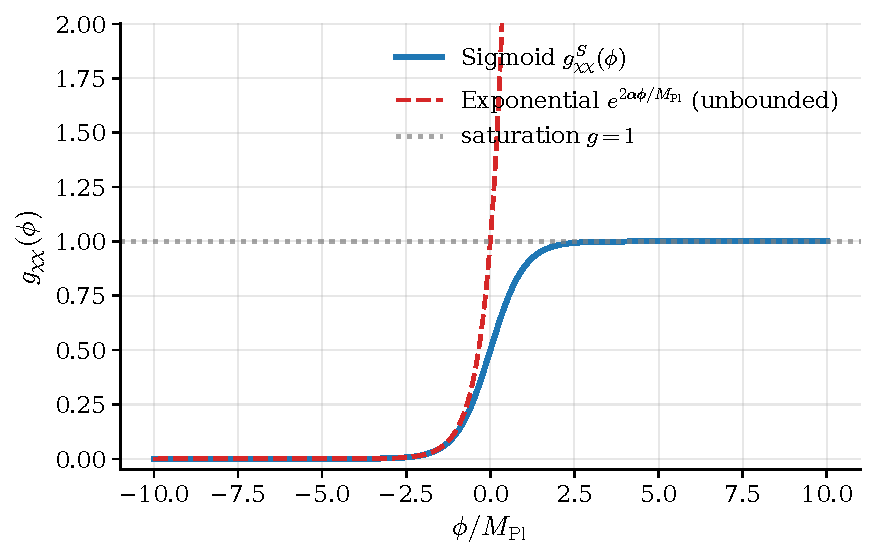
\includegraphics[width=0.78\textwidth]{figures/fsg_a_metric.pdf}
    \caption{\textbf{Field-space geometry, panel (a): sigmoid vs.\ exponential metric.}
        The sigmoid $g^S_{\chi\chi}(\phi) = (1+e^{-2\alpha\phi/M_{\rm Pl}})^{-1}$
        (blue) saturates at $g=1$ for $\phi \gg M_{\rm Pl}/\alpha$ while
        decaying to zero for $\phi \ll -M_{\rm Pl}/\alpha$, bounded by
        construction on both sides.  The bare exponential $e^{2\alpha\phi/M_{\rm Pl}}$
        (red dashed) grows without bound, which breaks perturbative
        unitarity during inflation.}
    \label{fig:field_space_geometry}
    \label{fig:fsg_metric}
\end{figure}

\begin{figure}[htbp]
    \centering
    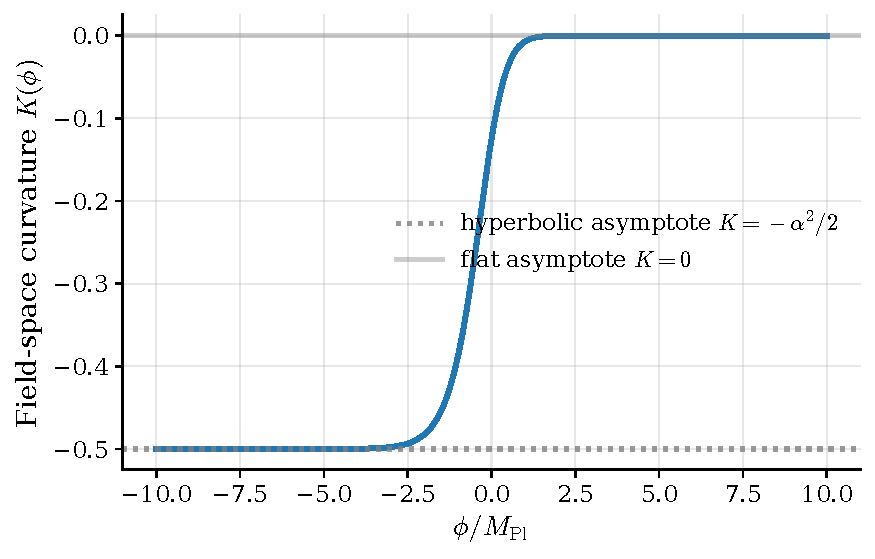
\includegraphics[width=0.78\textwidth]{figures/fsg_b_curvature.pdf}
    \caption{\textbf{Field-space geometry, panel (b): curvature transition.}
        The field-space scalar curvature $K(\phi) = -\tfrac{1}{2}\alpha^2
        (1 - g_{\chi\chi})^2$ transitions smoothly from its hyperbolic
        asymptote $K = -\alpha^2/2$ for $\phi \ll -M_{\rm Pl}/\alpha$
        (where the sigmoid regularization reproduces Poincar\'e
        $\alpha$-attractor geometry) to flat Euclidean $K = 0$ for
        $\phi \gg M_{\rm Pl}/\alpha$ (where the sigma model decouples).}
    \label{fig:fsg_curvature}
\end{figure}

\begin{figure}[htbp]
    \centering
    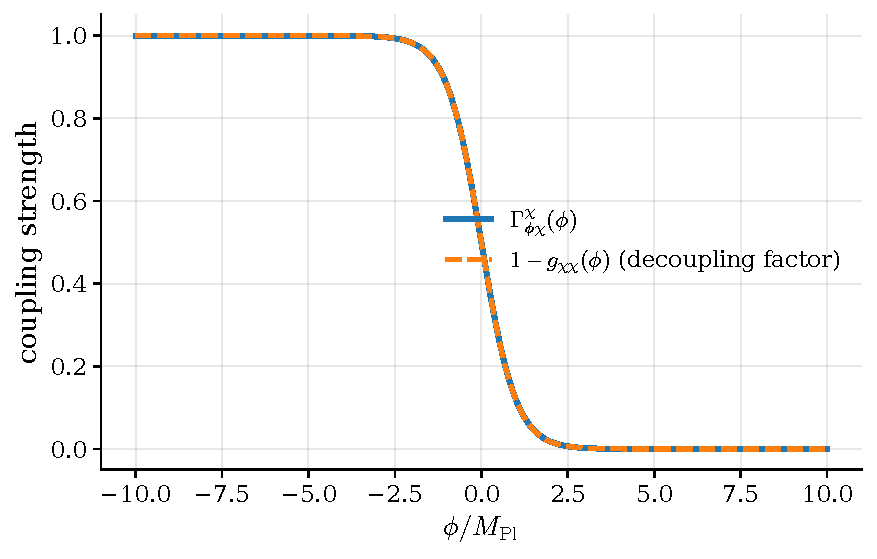
\includegraphics[width=0.78\textwidth]{figures/fsg_c_decoupling.pdf}
    \caption{\textbf{Field-space geometry, panel (c): decoupling factor.}
        The Christoffel symbol $\Gamma^\chi_{\phi\chi}(\phi) = (\alpha/M_{\rm Pl})(1-g_{\chi\chi})$
        (blue) and the decoupling factor $1 - g_{\chi\chi}$ (orange) both
        vanish as $g \to 1$, isolating the spectator $\chi$ from the inflaton
        $\phi$ on the inflationary plateau where observables are generated.}
    \label{fig:fsg_decoupling}
\end{figure}

We now present the derivation of the sigmoid metric with explicit classification of each logical step. We use three epistemic categories:

\begin{itemize}
\item \textbf{Theorem}: A mathematical consequence that follows necessarily from stated premises. No freedom of choice.
\item \textbf{Assumption}: A physically motivated condition imposed on the model. Could in principle be relaxed, leading to different models.
\item \textbf{Minimal Complexity Choice}: A selection among mathematically equivalent alternatives via a minimal-complexity principle. Different choices lead to the same qualitative physics but different quantitative details.
\end{itemize}

%------------------------------------------------------------------------------
\subsection{Boundary Conditions from Physical Principles}
%------------------------------------------------------------------------------

\begin{assumption_box}
\textbf{Condition 1 (Bounce Mechanism):} During the contracting phase ($\phi \ll 0$), the field space metric must exponentially suppress the kinetic energy of $\chi$:
\begin{equation}
\lim_{\phi \to -\infty} g_{\chi\chi}(\phi) \sim e^{2\alpha\phi/M_{\rm Pl}} \to 0.
\label{eq:cond1}
\end{equation}
\textit{Justification}: Without kinetic suppression, $\chi$ kinetic energy dominates the energy budget during contraction, preventing spatial curvature from triggering the bounce at sub-Planckian densities. This is a physical requirement for the bounce mechanism within standard GR.
\end{assumption_box}

\begin{assumption_box}
\textbf{Condition 2 (Perturbative Unitarity):} During inflation ($\phi \gg 0$), the kinetic terms must approach canonical form:
\begin{equation}
\lim_{\phi \to +\infty} g_{\chi\chi}(\phi) = 1 \quad (\text{canonical normalization}).
\label{eq:cond2}
\end{equation}
\textit{Justification}: Violation leads to exponential growth of kinetic energy, strong coupling, and breakdown of the perturbative description. The value 1 (rather than another finite constant) is a normalization convention.
\end{assumption_box}

\begin{assumption_box}
\textbf{Condition 3 (Ghost-Freedom):} The metric must be positive-definite:
\begin{equation}
g_{\chi\chi}(\phi) > 0 \quad \forall \phi \in \mathbb{R}.
\label{eq:cond3}
\end{equation}
\textit{Justification}: Zero or negative metric introduces ghost degrees of freedom (wrong-sign kinetic terms), rendering the theory unstable. Strict positivity also ensures that the field-space metric is non-degenerate ($\det G_{ab} = g_{\chi\chi} \neq 0$), so the kinetic sector remains invertible everywhere.
\end{assumption_box}

These three conditions constitute the \emph{physical input}. Everything that follows is either a mathematical consequence of these conditions or a minimal-complexity choice among solutions satisfying them.

%------------------------------------------------------------------------------
\subsection{Derivation of the Sigmoid Function}
%------------------------------------------------------------------------------

\begin{occam_box}
\textbf{Choice A (Autonomous ODE):} We seek $g(\phi)$ satisfying an autonomous first-order ODE: $dg/d\phi = f(g)$, where $f$ depends only on $g$, not explicitly on $\phi$.

\textit{Justification}: The boundary conditions \eqref{eq:cond1}--\eqref{eq:cond3} constrain only the limiting behavior of $g$, not its dependence on specific values of $\phi$. An autonomous equation is the simplest structure consistent with this. Non-autonomous choices $f(g, \phi)$ would introduce additional free functions without physical motivation.

\textit{Alternatives}: Any non-autonomous ODE $dg/d\phi = f(g, \phi)$ with the same boundary conditions would also work, but introduces arbitrary $\phi$-dependence.
\end{occam_box}

\begin{theorem_box}
\textbf{Consequence of Conditions 1--3 and Choice A:} The function $f(g)$ must satisfy $f(0) = f(1) = 0$ (fixed points at the boundary values) with $f(g) > 0$ for $g \in (0,1)$.

\textit{Proof}: Condition 1 requires $g \to 0$ as $\phi \to -\infty$, so $g=0$ must be a fixed point: $f(0) = 0$. Condition 2 requires $g \to 1$ as $\phi \to +\infty$, so $f(1) = 0$. It remains to show $f(g) > 0$ on $(0,1)$. For the autonomous ODE $dg/d\phi = f(g)$, any zero $f(g_*) = 0$ with $g_* \in (0,1)$ creates a fixed point that the trajectory cannot cross (by ODE uniqueness). Since the trajectory must connect $g=0$ to $g=1$, $f$ can have no interior zeros. Continuity then forces $f$ to maintain a constant sign on $(0,1)$; the sign must be positive because $g$ increases from $0$ to $1$. $\square$
\end{theorem_box}

\begin{occam_box}
\textbf{Choice B (Minimal Polynomial):} Among all functions $f(g)$ with zeros at $g=0$ and $g=1$ and $f > 0$ on $(0,1)$, we select the minimal-degree polynomial:
\begin{equation}
f(g) = C \cdot g^a (1-g)^b, \quad a, b > 0.
\end{equation}
We further choose $a = b = 1$ (simplest exponents):
\begin{equation}
\boxed{\frac{dg}{d\phi} = \frac{2\alpha}{M_{\rm Pl}} \cdot g(1-g)}
\label{eq:logistic}
\end{equation}

\textit{Justification}: This is a \textbf{minimal-complexity choice}, not a theorem. Any $(a,b) > 0$ produces a solution with the correct boundary conditions. The choice $a = b = 1$ yields the logistic equation, which has the additional property of producing the unique solution with the fastest approach to both boundaries (no flat intermediate plateaus). Different $(a,b)$ yield generalized logistic functions that would produce qualitatively identical bouncing cosmology with quantitatively similar predictions, because during inflation ($g \to 1$) and during contraction ($g \to 0$), all solutions converge to the same asymptotic behavior.

\textit{Physical consequences of other choices}: For $a = b = 2$, the sigmoid transition is slower. For $a=1, b=2$, the approach to the inflationary limit $g \to 1$ is faster. All choices satisfy Conditions 1--3 and produce viable bouncing cosmology.
\end{occam_box}

\begin{theorem_box}
\textbf{Unique Solution of the Logistic Equation:} Given Eq.~\eqref{eq:logistic} with the natural boundary condition $g(0) = 1/2$ (midpoint at $\phi = 0$):
\begin{equation}
\boxed{g_{\chi\chi}^S(\phi) = \frac{1}{1 + e^{-2\alpha\phi/M_{\rm Pl}}}}
\label{eq:sigmoid}
\end{equation}
\textit{Proof}: Standard separation of variables of the logistic equation. The boundary condition $g(0) = 1/2$ fixes the integration constant. Choosing $g(\phi_0) = 1/2$ for $\phi_0 \neq 0$ merely shifts $\phi$ by a constant. $\square$
\end{theorem_box}

%------------------------------------------------------------------------------
\subsection{Independent Geometric Derivation}
%------------------------------------------------------------------------------

The sigmoid metric also arises naturally from compactifying the Poincar\'e half-plane, providing geometric support independent of the complexity-based derivation.

\begin{theorem_box}
\textbf{Compactification of Hyperbolic Space:} Cosmological $\alpha$-attractors \cite{Kallosh2013,Carrasco2015} use the Poincar\'e half-plane metric $ds^2 = (dx^2 + dy^2)/y^2$. The transformation $y = e^{\alpha\phi/M_{\rm Pl}}$ yields $g_{\chi\chi} = e^{2\alpha\phi}$. The canonical compactification of $y \in (0,\infty)$ to $(0,1]$ via $g = y^2/(1+y^2)$ gives:
\begin{equation}
g = \frac{e^{2\alpha\phi/M_{\rm Pl}}}{1 + e^{2\alpha\phi/M_{\rm Pl}}} = \frac{1}{1 + e^{-2\alpha\phi/M_{\rm Pl}}} \quad \checkmark
\end{equation}
\textit{Note}: The map $g = y^2/(1+y^2)$ is a minimal-complexity choice among compactifications. Other choices (e.g., $g = \tanh^2(\alpha\phi)$) yield different regularizations with the same boundary behavior.
\end{theorem_box}

%------------------------------------------------------------------------------
\subsection{Summary of Epistemic Status}
\label{sec:epistemic_summary}
%------------------------------------------------------------------------------

\begin{table}[htbp]
\centering
\begin{tabular}{lcl}
\toprule
\textbf{Step} & \textbf{Status} & \textbf{Consequence if Changed} \\
\midrule
Condition 1 (suppression) & Assumption & No bounce mechanism \\
Condition 2 (saturation) & Assumption & Unitarity breakdown \\
Condition 3 (positivity) & Assumption & Ghost instability \\
$f(0)=f(1)=0$, $f>0$ & Theorem & (follows from above) \\
Autonomous ODE & Min.\ Complexity & Adds free function $f(\phi)$ \\
$a=b=1$ in $g^a(1-g)^b$ & Min.\ Complexity & Generalized logistic; same physics \\
$g(0)=1/2$ & Convention & Shifts $\phi$ origin \\
Sigmoid solution & Theorem & (follows from above) \\
Compactification $y^2/(1+y^2)$ & Min.\ Complexity & Different regularization; same asymptotics \\
\bottomrule
\end{tabular}
\caption{Epistemic classification of each step in the sigmoid metric derivation.}
\label{tab:epistemic}
\end{table}

The key message: the \textbf{three boundary conditions} (Assumptions) are the physical content. The sigmoid is the \textbf{simplest solution} satisfying them, selected by minimal complexity. Any other solution with the same boundary conditions would produce a qualitatively identical bouncing cosmology with the same asymptotic predictions ($n_s$, $r$), because these observables are determined by the inflationary regime where $g_{\chi\chi} \to 1$ regardless of the specific interpolation.

%==============================================================================
\section{The Complete Cosmological Model}
\label{sec:model}
%==============================================================================

\begin{figure}[htbp]
    \centering
    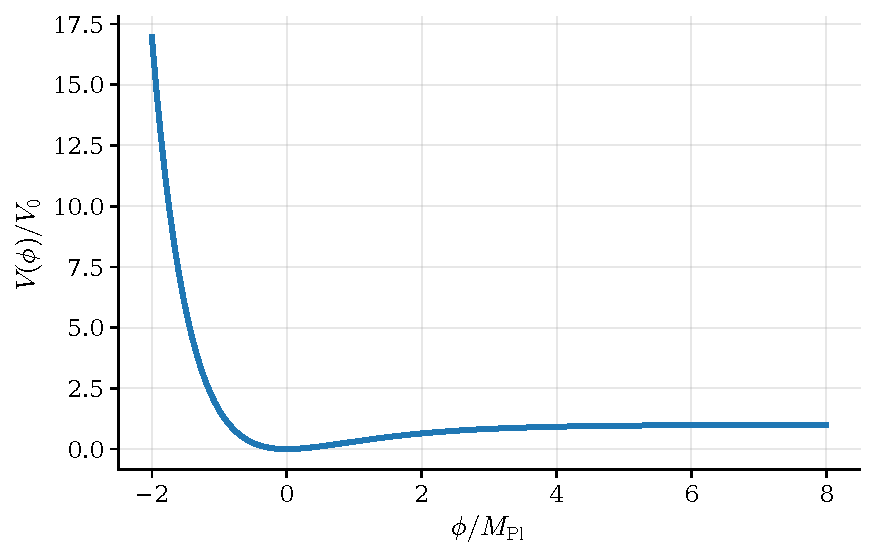
\includegraphics[width=0.78\textwidth]{figures/pd_a_potential.pdf}
    \caption{\textbf{Potential and dynamics, panel (a): Starobinsky potential.}
        $V(\phi) = V_0\,(1 - e^{-\beta\phi/M_{\rm Pl}})^2$ in units of $V_0$.
        The plateau at $\phi \gg M_{\rm Pl}$ supports many e-folds of slow-roll
        inflation; the steep drop near $\phi \sim 0$ ends inflation at
        $\phi_{\rm end} \approx 0.94\,M_{\rm Pl}$.}
    \label{fig:potential_dynamics}
    \label{fig:pd_potential}
\end{figure}

\begin{figure}[htbp]
    \centering
    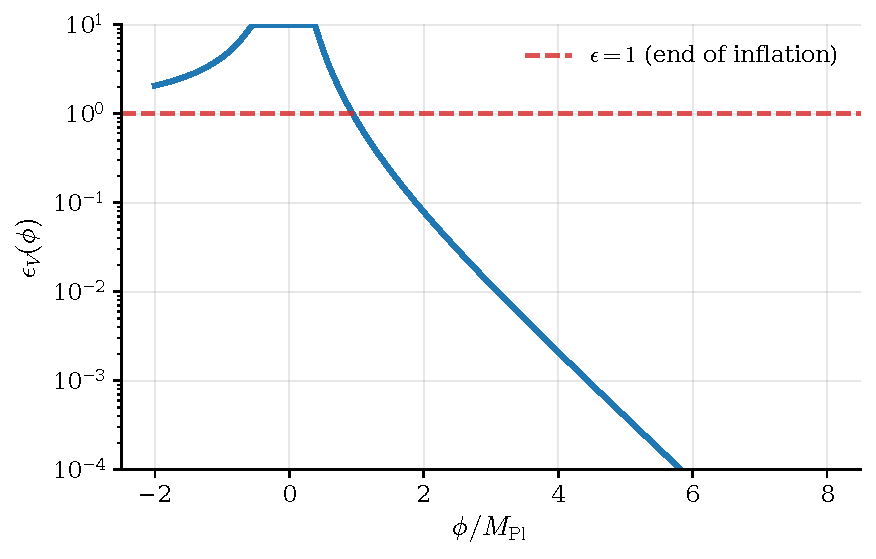
\includegraphics[width=0.78\textwidth]{figures/pd_b_epsilon.pdf}
    \caption{\textbf{Potential and dynamics, panel (b): slow-roll parameter.}
        $\epsilon_V(\phi) = \tfrac{1}{2}M_{\rm Pl}^2 (V'/V)^2$.  Slow-roll
        ($\epsilon_V \ll 1$) holds throughout the plateau; the dashed line
        at $\epsilon_V = 1$ marks the end-of-inflation condition used
        to define $\phi_{\rm end}$.}
    \label{fig:pd_epsilon}
\end{figure}

\begin{figure}[htbp]
    \centering
    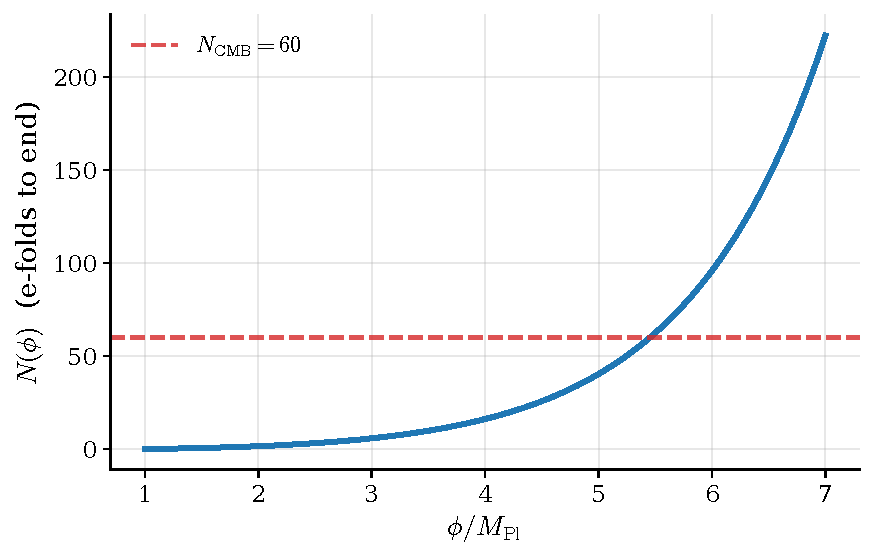
\includegraphics[width=0.78\textwidth]{figures/pd_c_efolds.pdf}
    \caption{\textbf{Potential and dynamics, panel (c): e-folds to end of inflation.}
        $N(\phi) = \tfrac{3}{4}(e^{\beta\phi} - e^{\beta\phi_{\rm end}})
        - (\phi - \phi_{\rm end})/(2\beta)$ with $\beta = \sqrt{2/3}$.
        The CMB pivot at $N_{\rm CMB} = 60$ corresponds to
        $\phi_{\rm CMB} \approx 5.45\,M_{\rm Pl}$ (full slow-roll inversion;
        see Section~\ref{sec:flatness}).}
    \label{fig:pd_efolds}
\end{figure}

\begin{figure}[htbp]
    \centering
    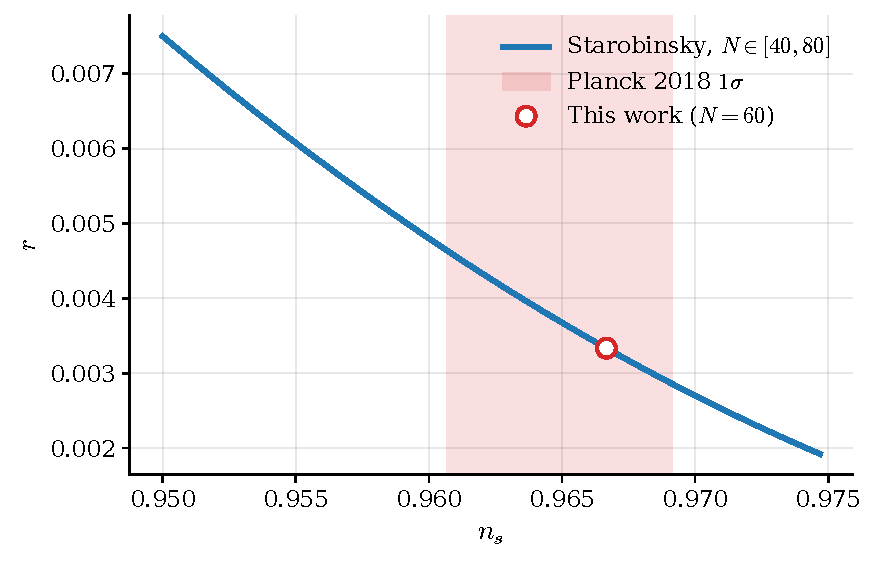
\includegraphics[width=0.78\textwidth]{figures/pd_d_ns_r.pdf}
    \caption{\textbf{Potential and dynamics, panel (d): $n_s$--$r$ plane.}
        Starobinsky prediction over $N\in[40,80]$ (blue curve), with the
        Planck~2018 $1\sigma$ band on $n_s$ (red).  This work, evaluated at
        $N=60$, sits well within the band at $(n_s,r) = (\nsAnalytical,
        \rAnalytical)$.}
    \label{fig:pd_ns_r}
\end{figure}

\subsection{Action and Field Space Geometry}

We consider a two-field model:
\begin{equation}
S = \int d^4x \sqrt{-g} \left[ \frac{M_{\rm Pl}^2}{2} R - \frac{1}{2} G_{ab} \nabla_\mu \phi^a \nabla^\mu \phi^b - V(\phi,\chi) \right],
\end{equation}
with field space metric $G_{ab} = \text{diag}(1, g_{\chi\chi}(\phi))$, $g_{\chi\chi}(\phi) = (1 + e^{-2\alpha\phi/M_{\rm Pl}})^{-1}$, and the Starobinsky potential $V = V_0(1 - e^{-\beta\phi/M_{\rm Pl}})^2 + \frac{1}{2}m_\chi^2\chi^2$ with $\beta = \sqrt{2/3}$, $V_0 = 10^{-10} M_{\rm Pl}^4$.

\subsection{Background Evolution in Closed Universe}

The Friedmann equations for $k=+1$:
\begin{align}
H^2 &= \frac{\rho}{3M_{\rm Pl}^2} - \frac{1}{a^2}, \label{eq:friedmann} \\
\dot{H} &= -\frac{\rho+p}{2M_{\rm Pl}^2} + \frac{1}{a^2}, \label{eq:acceleration}
\end{align}
where $\rho = \frac{1}{2}\dot\phi^2 + \frac{1}{2}g_{\chi\chi}\dot\chi^2 + V$, $p = \frac{1}{2}\dot\phi^2 + \frac{1}{2}g_{\chi\chi}\dot\chi^2 - V$.

The NEC is satisfied throughout: $\rho + p = \dot\phi^2 + g_{\chi\chi}\dot\chi^2 \geq 0$.

The bounce occurs when $H = 0$, i.e., $\rho = 3M_{\rm Pl}^2/a^2$. Since kinetic energy is subdominant near the bounce ($\dot\phi^2 \ll V$ on the slow-roll plateau), $\rho \approx V_0$ and the bounce scale is set by
\begin{equation}
a_{\rm min} \approx \sqrt{\frac{3 M_{\rm Pl}^2}{V_0}} \approx 1.73 \times 10^5 \, M_{\rm Pl}^{-1},
\label{eq:a_bounce}
\end{equation}
which we denote $a_{\rm min}$ (equivalently $a_{\rm bounce}$). This relation connects the inflationary energy scale $V_0$ directly to the bounce geometry: a lower $V_0$ produces a larger $a_{\rm min}$ and thus a weaker spatial curvature at the bounce. The Hubble scale during inflation, $H_{\rm inf} \approx \sqrt{V_0/(3M_{\rm Pl}^2)} \approx 5.8 \times 10^{-6}\,M_{\rm Pl}$, is the reciprocal: $H_{\rm inf} \approx 1/a_{\rm min}$.

Note that $g_{\chi\chi}$ appears in the kinetic terms of both $\rho$ and $p$. For $\phi \gg M_{\rm Pl}/\alpha$, $g_{\chi\chi} \to 1$ and the background equations reduce to the standard two-field form. The saturation threshold depends on $\alpha$: for the fiducial $\alpha = 1$ at $\phi_{\rm bounce} \approx 10\,M_{\rm Pl}$, $|1 - g_{\chi\chi}| < 10^{-9}$, while for $\alpha = 0.1$ at $\phi_{\rm CMB} \approx 5.4\,M_{\rm Pl}$, $g_{\chi\chi} \approx 0.74$. Nevertheless, observable predictions are $\alpha$-independent: on the baseline $\chi = \dot\chi = 0$ trajectory $g_{\chi\chi}$ decouples from the Friedmann and Klein-Gordon equations regardless of its value, and a separate nontrivial spectator-displacement scan confirms that the universality is not a tautology of this kinematic choice (Section~\ref{sec:observables}).

\begin{assumption_box}
\textbf{Initial conditions.} We initialize the contracting phase with $\phi_0 \approx 10 M_{\rm Pl}$ on the Starobinsky plateau, $\dot\phi_0 = 0$, and the scale factor at $a_0 = 1.8\,a_{\rm min}$ above the bounce minimum. The origin of these initial conditions---how the universe enters a contracting phase with the inflaton on the slow-roll plateau---is not addressed here and is a common open question in bouncing cosmologies \cite{Novello2008}.

\textbf{Hubble anti-friction during contraction.} During contraction ($H < 0$), the $3H\dot\phi$ term in the Klein-Gordon equation acts as anti-friction, amplifying kinetic energy as $\dot\phi^2 \propto a^{-6}$. Any small deviation from $\dot\phi = 0$ grows rapidly, potentially destroying slow roll and the conditions for a curvature-driven bounce. This is a fundamental limitation of $w \approx -1$ contraction (ekpyrotic models with $w \gg 1$ avoid this by making contraction an attractor). In our model, the contraction spans only $\Delta N = \ln(1.8) \approx 0.59$ e-folds, so kinetic energy amplification is bounded by $a_0^6/a_{\rm min}^6 = 1.8^6 \approx 34$. Starting from $\dot\phi_0 = 0$, the potential gradient generates $\dot\phi \sim V'\Delta t$, which remains negligible over this short interval. The fine-tuning required is thus modest: initial kinetic energy must satisfy $\frac{1}{2}\dot\phi_0^2 \lesssim 34^{-1} V_0 \sim 3 \times 10^{-12}$, which is automatically satisfied for $\dot\phi_0 = 0$. However, we do not explain \emph{why} the universe begins contracting with near-zero kinetic energy on the plateau; this remains an open question, shared with all bouncing cosmologies. We emphasize that the fine-tuning is \emph{quantitatively modest}: starting with any $\dot\phi_0^2 \lesssim 3 \times 10^{-12}\,M_{\rm Pl}^4$ (i.e., kinetic energy below $\sim 3\%$ of $V_0$) suffices for a successful bounce. This is a single inequality on one initial datum, comparable to the flatness requirement in standard inflation. A cyclic extension, in which the turnaround mechanism naturally deposits the inflaton on the plateau with near-zero velocity, would eliminate this condition entirely.

\textbf{Gradient stability of the contraction phase.} Gradient perturbations $\delta\rho/\rho \propto k^2/(a^2\rho)$ also grow during $w \approx -1$ contraction. Over $\Delta N \approx 0.59$ e-folds, they amplify by $\lesssim e^{2\Delta N} \approx 3.2$, insufficient for nonlinear growth. The brevity of contraction (set by the large bounce scale $a_{\rm min} \sim 10^5\,M_{\rm Pl}^{-1}$) prevents both the Hubble anti-friction and gradient instabilities from developing.
\end{assumption_box}

%==============================================================================
\section{Numerical Validation and Robustness}
\label{sec:numerics}
%==============================================================================

\begin{figure}[htbp]
    \centering
    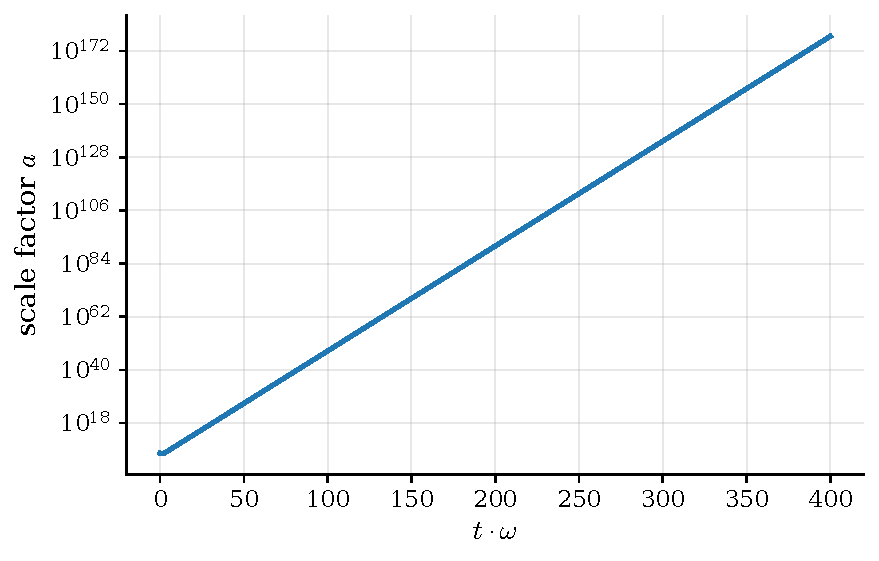
\includegraphics[width=0.78\textwidth]{figures/bg_a_scale_factor.pdf}
    \caption{\textbf{Background evolution, panel (a): scale factor.}
        $a(t)$ on a log scale through the contracting and expanding phases.
        The minimum at the bounce ($a = a_{\rm min} \approx \aMinBounce\,M_{\rm Pl}^{-1}$,
        Eq.~\ref{eq:a_bounce}) is non-singular; thereafter Starobinsky
        inflation provides $\NpostBounce$ post-bounce e-folds within the
        simulated window.}
    \label{fig:background_evolution}
    \label{fig:bg_scale_factor}
\end{figure}

\begin{figure}[htbp]
    \centering
    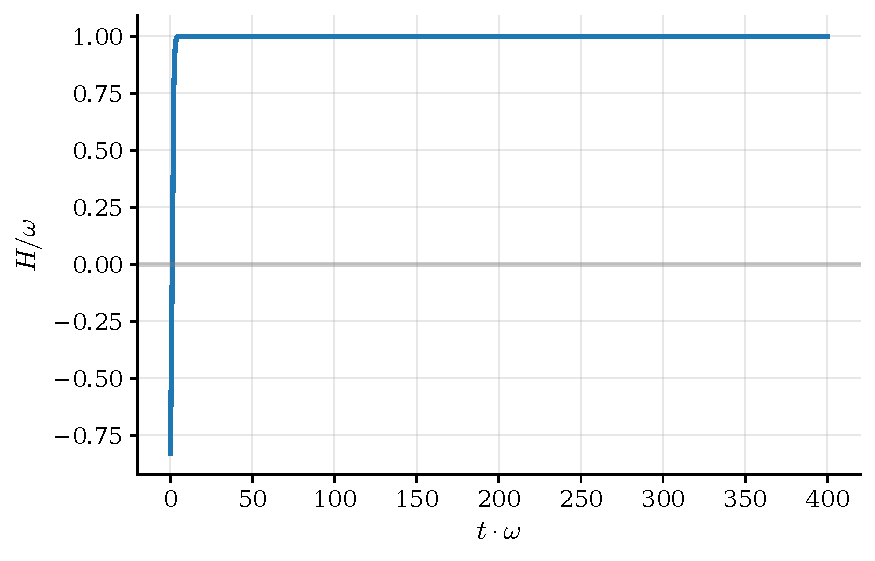
\includegraphics[width=0.78\textwidth]{figures/bg_b_hubble.pdf}
    \caption{\textbf{Background evolution, panel (b): Hubble parameter.}
        $H(t)$ in units of $\omega = \sqrt{V_0/(3M_{\rm Pl}^2)}$, passing
        smoothly through $H = 0$ at the bounce.  Newtonian-gauge
        perturbations remain finite at this point (Section~\ref{sec:perturbations}).}
    \label{fig:bg_hubble}
\end{figure}

\begin{figure}[htbp]
    \centering
    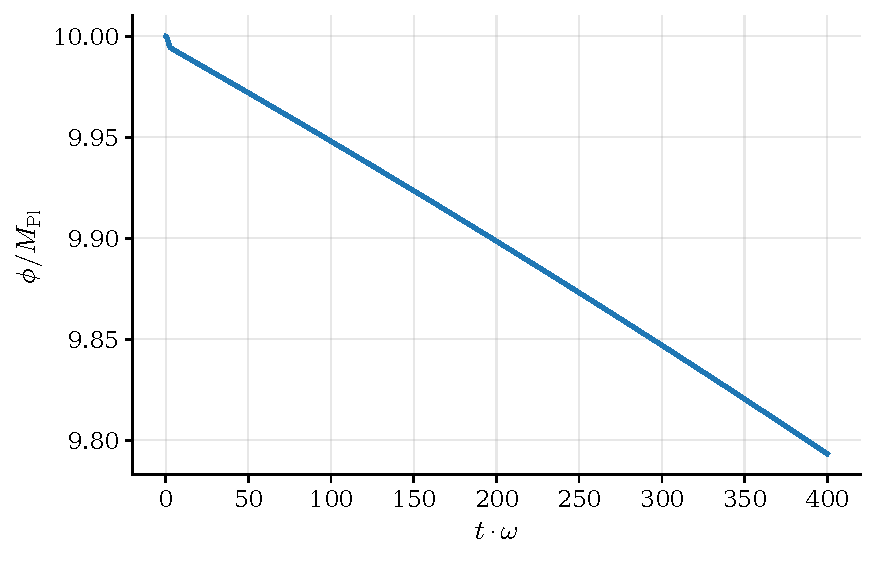
\includegraphics[width=0.78\textwidth]{figures/bg_c_inflaton.pdf}
    \caption{\textbf{Background evolution, panel (c): inflaton field $\phi(t)$.}
        Initialized at $\phi_0 \approx 10\,M_{\rm Pl}$ on the Starobinsky plateau,
        $\phi$ remains essentially flat through the brief contraction and
        bounce, then slow-rolls to $\phi_{\rm end} \approx 0.94\,M_{\rm Pl}$
        over $\sim\bumpNtotal$ post-bounce e-folds.}
    \label{fig:bg_inflaton}
\end{figure}

\begin{figure}[htbp]
    \centering
    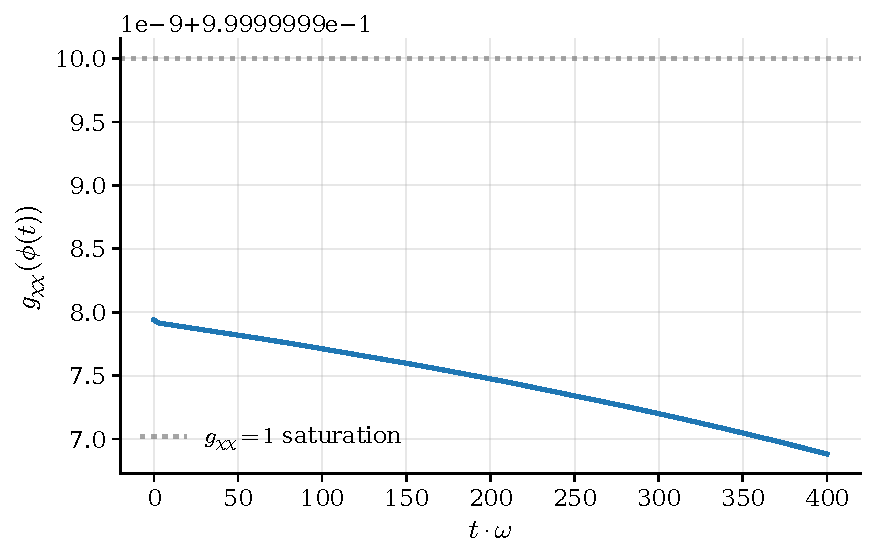
\includegraphics[width=0.78\textwidth]{figures/bg_d_metric.pdf}
    \caption{\textbf{Background evolution, panel (d): field-space metric saturation.}
        $g_{\chi\chi}(\phi(t))$ saturates to unity within a few e-folds after the
        bounce: by the time CMB-relevant perturbation modes exit the
        Hubble radius, $|1 - g_{\chi\chi}| < \gDeviationMax$ (essentially
        canonical kinetic terms).}
    \label{fig:bg_metric}
\end{figure}

\begin{figure}[htbp]
    \centering
    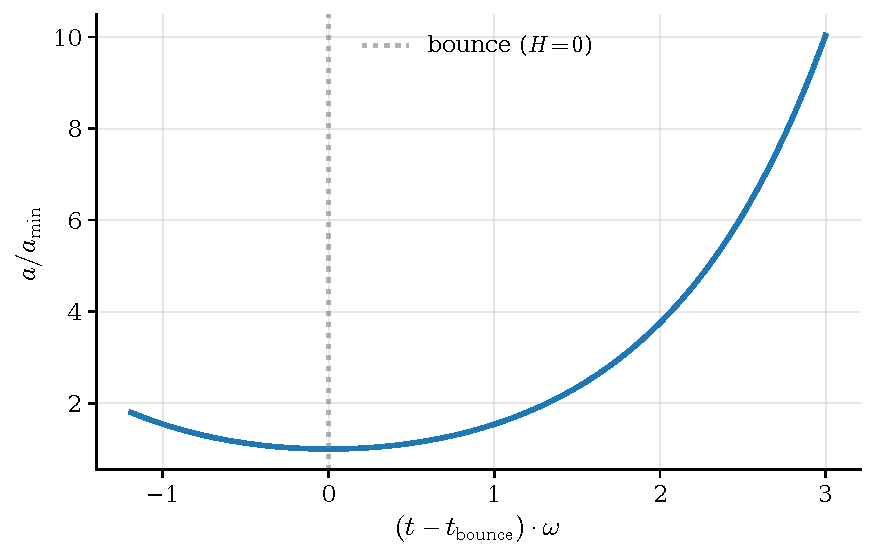
\includegraphics[width=0.78\textwidth]{figures/bz_a_scale_factor.pdf}
    \caption{\textbf{Bounce region, panel (a): scale factor near $a_{\rm min}$.}
        Zoom around the bounce point.  $a(t)$ is smooth and parabolic at the
        minimum; no singular behaviour.}
    \label{fig:bounce_zoom}
    \label{fig:bz_scale_factor}
\end{figure}

\begin{figure}[htbp]
    \centering
    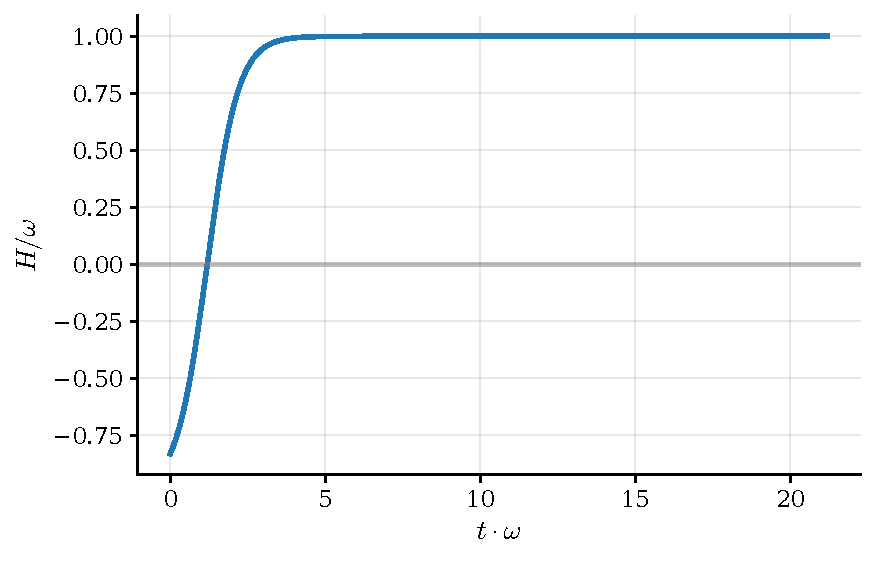
\includegraphics[width=0.78\textwidth]{figures/bz_b_hubble.pdf}
    \caption{\textbf{Bounce region, panel (b): Hubble parameter through $H = 0$.}
        $H(t)$ crosses zero linearly at the bounce, with $\dot H$ finite
        and continuous.}
    \label{fig:bz_hubble}
\end{figure}

\begin{figure}[htbp]
    \centering
    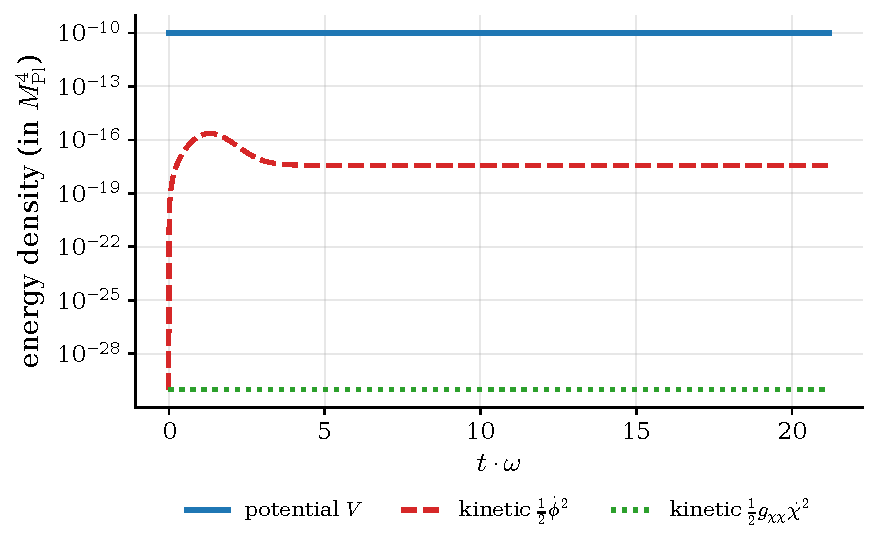
\includegraphics[width=0.78\textwidth]{figures/bz_c_energies.pdf}
    \caption{\textbf{Bounce region, panel (c): energy components.}
        Near the bounce the potential $V$ (blue) dominates over both
        $\tfrac{1}{2}\dot\phi^2$ (red dashed) and the $\chi$ kinetic
        contribution $\tfrac{1}{2}g_{\chi\chi}\dot\chi^2$ (green dotted,
        negligible on the fiducial $\chi=\dot\chi=0$ trajectory).
        This is what makes spatial curvature, not kinetic energy, set the
        bounce scale.}
    \label{fig:bz_energies}
\end{figure}

\begin{figure}[htbp]
    \centering
    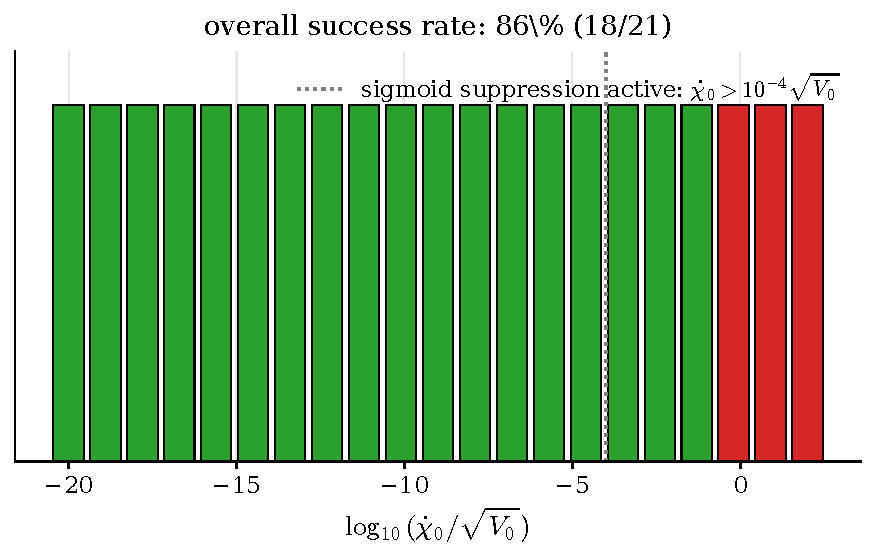
\includegraphics[width=0.78\textwidth]{figures/ba_a_success_map.pdf}
    \caption{\textbf{Basin of attraction, panel (a): success map vs.\ initial $\dot\chi_0$.}
        Successful bounces (green) versus failures (red) across 22 orders
        of magnitude in $\dot\chi_0$ ($10^{-20}\sqrt{V_0}$ to $10^{+2}\sqrt{V_0}$).
        Sigmoid suppression of $\chi$-kinetic energy becomes operationally
        important above the dotted line at $\dot\chi_0 \sim 10^{-4}\sqrt{V_0}$.}
    \label{fig:basin_attraction}
    \label{fig:ba_success_map}
\end{figure}

\begin{figure}[htbp]
    \centering
    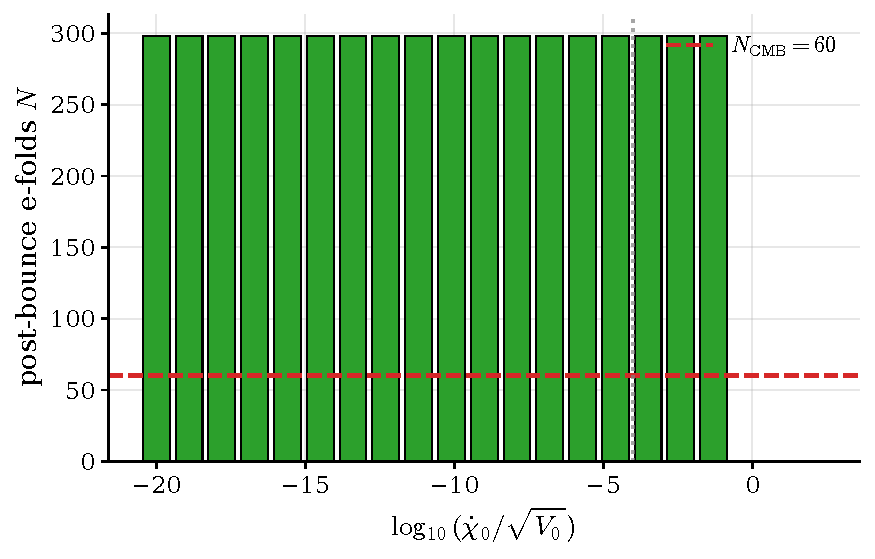
\includegraphics[width=0.78\textwidth]{figures/ba_b_efolds.pdf}
    \caption{\textbf{Basin of attraction, panel (b): post-bounce e-folds.}
        For each successful bounce, the number of post-bounce e-folds
        achieved before integration end.  All small-$\dot\chi_0$ runs
        comfortably exceed the $N_{\rm CMB} = 60$ requirement.}
    \label{fig:ba_efolds}
\end{figure}

The sigmoid regularization achieves robust bounce and inflation across an extended range of initial $\dot\chi$ spanning 22 orders of magnitude ($10^{-20}$ to $10^{+2}$ in units of $\sqrt{V_0}$), with an overall success rate of $86\%$ (18/21 representative samples). For the small-$\dot\chi$ regime ($10^{-20}$ to $10^{-4}$), where $\chi$ is essentially inactive, 100\% success rate is achieved with $\sim 300$ post-bounce e-folds. For the large-$\dot\chi$ regime ($10^{-4}$ to $10^{+2}$), where the sigmoid suppression mechanism is actively required, $\sim 50\%$ of cases succeed---the failures correspond to initial kinetic energies that exceed the curvature-driven bounce capacity. Friedmann constraint is satisfied to relative error $< 10^{-6}$.

%==============================================================================
\section{Flatness Problem Resolution}
\label{sec:flatness}
%==============================================================================

\begin{figure}[htbp]
    \centering
    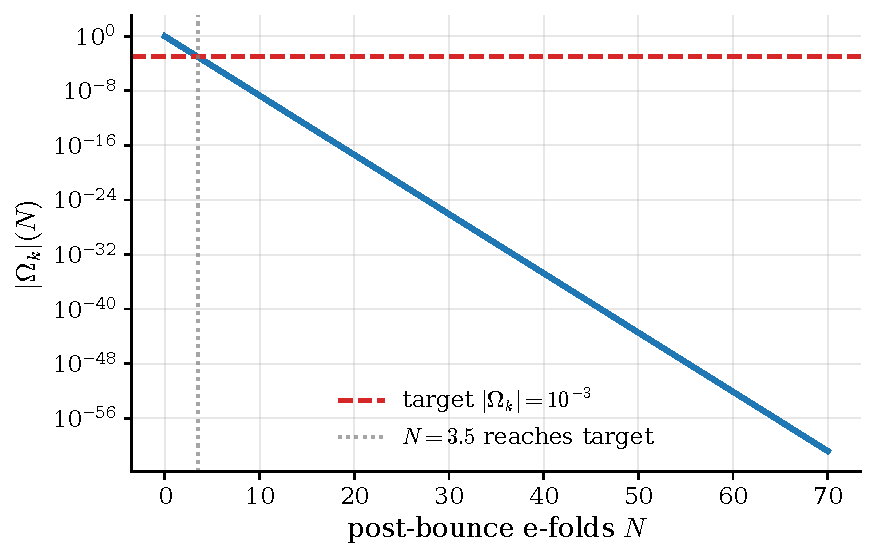
\includegraphics[width=0.78\textwidth]{figures/fl_a_dilution.pdf}
    \caption{\textbf{Curvature dilution, panel (a): $|\Omega_k|$ vs.\ post-bounce $N$.}
        Spatial curvature is diluted exponentially after the bounce:
        $|\Omega_k|(N) = (a_{\rm min}\,e^N\,H_{\rm inf})^{-2}$.  Only $N \gtrsim 3.5$
        e-folds are required to bring $|\Omega_k|$ below $10^{-3}$; the
        many post-bounce e-folds of subsequent inflation drive it
        exponentially below any observational bound.}
    \label{fig:flatness_evolution}
    \label{fig:fl_dilution}
\end{figure}

\begin{figure}[htbp]
    \centering
    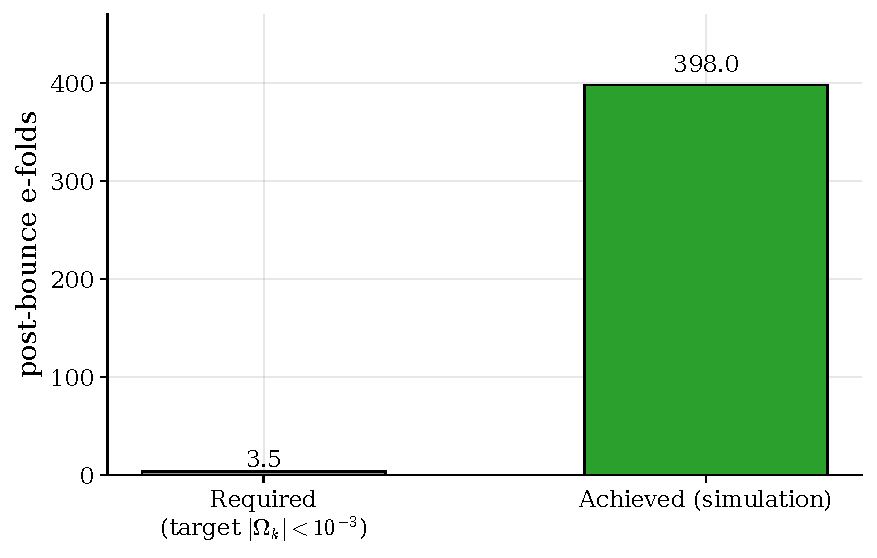
\includegraphics[width=0.78\textwidth]{figures/fl_b_compare.pdf}
    \caption{\textbf{Curvature dilution, panel (b): required vs.\ achieved e-folds.}
        Our integration produces $\NpostBounce$ post-bounce e-folds, two
        orders of magnitude beyond the $\sim 3.5$ needed for the flatness
        target.  By any standard cosmological measure the universe is
        spatially flat by the time CMB modes exit the Hubble radius.}
    \label{fig:fl_compare}
\end{figure}

After bounce at $a_{\rm min} \approx 1.73 \times 10^5 M_{\rm Pl}^{-1}$ with $H_{\rm inf} \approx 5.8 \times 10^{-6} M_{\rm Pl}$, only $N > 3.5$ e-folds are required to satisfy $|\Omega_k| < 0.001$. With 60+ e-folds, $|\Omega_k| \sim 10^{-52}$.

We distinguish three e-fold counts.  $N_{\rm total}$ is the total number of inflationary e-folds from the bounce to the end of slow roll, set by $\phi_{\rm bounce}$.  Two values appear throughout the paper, and we distinguish them explicitly to avoid confusion:
\begin{itemize}
  \item $N_{\rm total}^{\rm ideal} = 2635$ for $\phi_{\rm bounce} = 10\,M_{\rm Pl}$ \emph{exactly}, from the full slow-roll formula
  \begin{equation}
    N(\phi) = \tfrac{3}{4}\bigl(e^{\beta\phi} - e^{\beta\phi_{\rm end}}\bigr) - \frac{\phi - \phi_{\rm end}}{2\beta}, \qquad \phi_{\rm end} \approx 0.94\,M_{\rm Pl}
    \label{eq:Nofphi}
  \end{equation}
  (the leading $\tfrac{3}{4}e^{\beta\phi}$ term dominates for $\phi \gg M_{\rm Pl}$).  This is an analytical idealization for the initial-condition choice $\phi_0 = 10\,M_{\rm Pl}$ and is referenced once here.
  \item $N_{\rm total}^{\rm sim} = \bumpNtotal$ --- Eq.~\eqref{eq:Nofphi} evaluated at the simulation's recorded initial $\phi_0$ (which is the value the bump-fit diagnostic uses; it differs from the idealized $10\,M_{\rm Pl}$ by integrator-level discretization). The simulated trajectory is not integrated all the way to $\epsilon_V = 1$ within the perturbation window $t_{\max} = 400/\omega$, so $N_{\rm total}^{\rm sim}$ is itself an analytical Starobinsky extrapolation from the simulated initial condition rather than a count of integrated e-folds. Throughout the paper, all numerical figures and observable hierarchies refer to $N_{\rm total}^{\rm sim}$ via the macro $\bumpNtotal$ unless the surrounding text explicitly says ``idealized''.
\end{itemize}
$N_{\rm CMB} = 60$ is the number of e-folds from when CMB-scale modes exit the Hubble radius to the end of inflation.  The first $N_{\rm total}^{\rm sim} - N_{\rm CMB} = \NhiddenEfolds$ post-bounce e-folds are observationally inaccessible (or 2575 for the idealized $\phi_{\rm bounce}=10\,M_{\rm Pl}$), and the bounce-scale spectral feature at $k \sim k_H$ lies within this unobservable epoch.  Our perturbation integration covers $\NpostBounce$ e-folds after the bounce (bounded by the integration window $t_{\max} = 400/\omega$, where $\omega = \sqrt{V_0/(3M_{\rm Pl}^2)}$): well past horizon exit of every mode in the 16-mode sweep, but far short of the full $N_{\rm total}^{\rm sim}$ required to track CMB-pivot modes from the bounce to their horizon exit (Section~\ref{sec:cmb_verification} addresses CMB scales separately).

%==============================================================================
\section{BKL Compatibility: Dynamical Anisotropy Analysis}
\label{sec:bkl}
%==============================================================================

\begin{figure}[htbp]
    \centering
    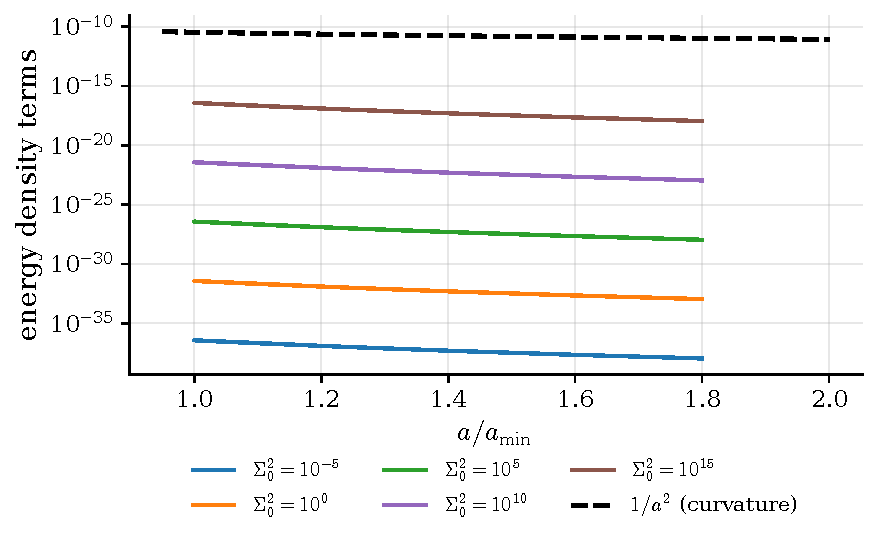
\includegraphics[width=0.78\textwidth]{figures/bkl_a_shear_vs_curv.pdf}
    \caption{\textbf{BKL analysis, panel (a): shear vs.\ curvature during contraction.}
        Shear energy density $\Sigma^2/a^6$ (coloured curves, one per
        initial $\Sigma_0^2$) compared against the spatial-curvature term
        $1/a^2$ (black dashed) on the approach to the bounce.  For all
        physically reasonable initial shear amplitudes
        ($\Sigma_0^2 \lesssim 10^{18}$), curvature dominates over shear at
        the bounce, so anisotropy never triggers a Kasner transition.}
    \label{fig:bkl_analysis}
    \label{fig:bkl_shear_vs_curv}
\end{figure}

\begin{figure}[htbp]
    \centering
    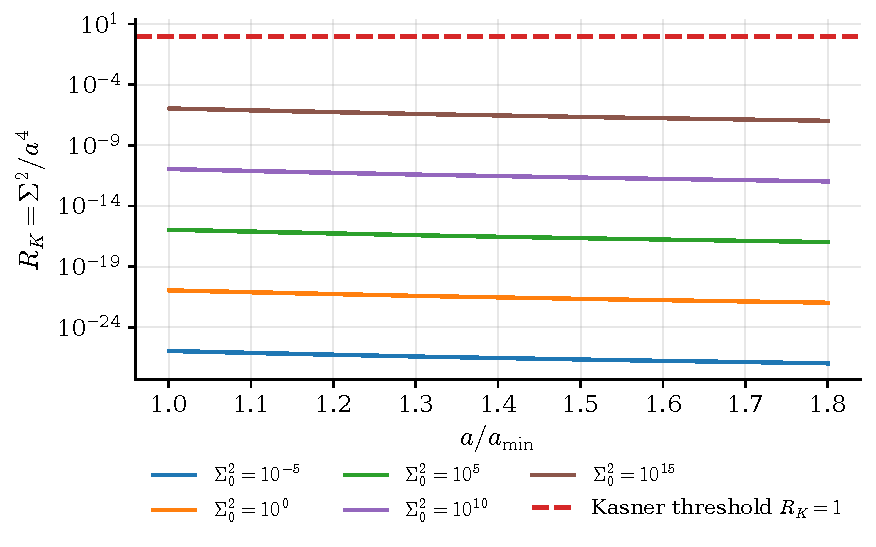
\includegraphics[width=0.78\textwidth]{figures/bkl_b_kasner_ratio.pdf}
    \caption{\textbf{BKL analysis, panel (b): Kasner ratio.}
        $R_K(a) = \Sigma^2/a^4$ as a function of scale factor $a/a_{\rm min}$
        through the contraction phase.  The Kasner threshold $R_K = 1$
        (red dashed) is the condition for chaotic Mixmaster behaviour;
        no curve crosses it, confirming that the wall-free truncation
        remains self-consistent for the entire scanned range.}
    \label{fig:bkl_kasner_ratio}
\end{figure}

\begin{figure}[htbp]
    \centering
    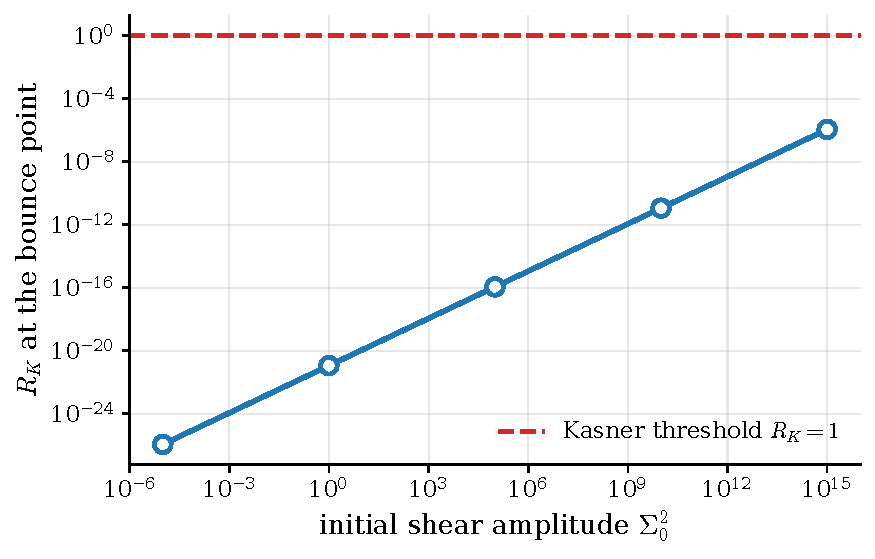
\includegraphics[width=0.78\textwidth]{figures/bkl_c_at_bounce.pdf}
    \caption{\textbf{BKL analysis, panel (c): bounce-point Kasner ratio vs.\ initial shear.}
        $R_K$ evaluated at the bounce, plotted against the initial shear
        amplitude $\Sigma_0^2$.  The relation is monotonic and crosses
        the threshold $R_K = 1$ (red dashed) only for unphysically large
        $\Sigma_0^2 \gtrsim a_{\rm min}^4 \sim 10^{20}$, far above any
        cosmologically reasonable value.}
    \label{fig:bkl_at_bounce}
\end{figure}

\subsection{Previous Analysis and Its Limitations}

In v3 \cite{Kravchenko2025v3}, we presented a static comparison: at the bounce scale $a_{\rm min} \approx 1.73 \times 10^5$, spatial curvature ($1/a^2$) dominates over shear ($\Sigma^2/a^6$) by many orders of magnitude. This argument, while correct, did not address whether the shear could \emph{grow dynamically} during contraction to the point where it triggers Kasner transitions (Mixmaster chaos).

\subsection{Kasner Transition Condition}

In Bianchi~IX cosmology, chaotic Mixmaster behavior \cite{Belinsky1970,Belinsky1982} occurs when anisotropic shear dominates over both matter and spatial curvature:
\begin{equation}
\frac{\Sigma^2}{a^6} > \frac{1}{a^2} \quad \Longrightarrow \quad \Sigma^2 > a^4.
\label{eq:kasner_condition}
\end{equation}
At our bounce scale, this requires $\Sigma^2 > a_{\rm min}^4 \approx 9 \times 10^{20} M_{\rm Pl}^4$---an enormous initial shear.

\subsection{Dynamical Evolution}

We numerically solve the Bianchi~IX equations with scalar field. The shear is characterized by the conserved quantity $\Sigma^2$, which enters the generalized Friedmann equations as:
\begin{align}
H^2 &= \frac{\rho}{3M_{\rm Pl}^2} - \frac{1}{a^2} + \frac{\Sigma^2}{6a^6}, \\
\dot{H} &= -\frac{\rho+p}{2M_{\rm Pl}^2} + \frac{1}{a^2} - \frac{\Sigma^2}{2a^6}.
\end{align}
Here $\Sigma^2$ is a \emph{constant of motion} in the absence of the Bianchi~IX anisotropy potential walls (the non-abelian curvature terms $\propto a^{-4}$ that drive Mixmaster oscillations). In the full Bianchi~IX dynamics, these walls cause $\Sigma^2$ to change during Kasner bounces; our truncation is valid when $\Sigma^2 \ll a_{\rm min}^4$, i.e., when shear never reaches the potential walls. The physical shear scalar $\sigma^2 = \Sigma^2/a^6$ satisfies $\tfrac{d}{dt}(\sigma^2) = -6H\sigma^2$. During contraction ($H < 0$), $a$ decreases and $\sigma^2$ grows, but $\Sigma^2$ is fixed.

\begin{theorem_box}
\textbf{Self-consistency of shear evolution:} The physical shear $\sigma^2 = \Sigma^2/a^6$ grows during contraction as $a$ decreases. The Kasner ratio is $R_K = \Sigma^2/a^4$. If the contraction is dominated by potential energy ($w \approx -1$), then $a \sim (t_b - t)^{1/3}$ and $R_K = \Sigma^2/a^4 \sim (t_b - t)^{-4/3} \to \infty$ as $t \to t_b$. This would seem problematic.

However, the key difference from BKL is that our bounce occurs at \emph{finite} $a_{\rm min} \gg l_{\rm Pl}$, not at $a \to 0$. The contraction phase from $a_0 \sim 1.8 a_{\rm min}$ to $a_{\rm min}$ involves only a factor of $\sim 1.8$ change in scale factor:
\begin{equation}
\frac{R_K(a_{\rm min})}{R_K(a_0)} = \left(\frac{a_0}{a_{\rm min}}\right)^4 \approx 1.8^4 \approx 10.5.
\end{equation}
Therefore, the Kasner ratio grows by at most a factor $\sim 10$ during contraction, while the Kasner threshold $\Sigma^2 > a_{\rm min}^4 \sim 10^{20}$ remains fixed.
\end{theorem_box}

\subsection{Numerical Results}

We solve the Bianchi~IX system for representative initial shear amplitudes covering 31 orders of magnitude: $\Sigma^2_0 \in [10^{-10}, 10^{21}]$ (in Planck units), including values \emph{above} the Kasner threshold $a_{\rm min}^4 \approx 9 \times 10^{20}$. The shear scalar $\Sigma^2$ is treated as a conserved parameter (not a dynamical variable): in the absence of Bianchi~IX potential walls, the shear contribution enters only through $\rho_\sigma = \Sigma^2/(2a^6)$ and $p_\sigma = \rho_\sigma$ in the Raychaudhuri equation, with $d\Sigma^2/dt = 0$ exactly. This is the standard treatment for the wall-free regime \cite{Erickson2004}; Kasner transitions (if they occur) would redistribute anisotropy among axes but are not modeled here. For all sub-threshold values:

\begin{itemize}
\item The Kasner ratio $R_K = \Sigma^2/a^4$ remains below unity throughout the contraction phase.
\item No Kasner transitions occur: the isotropic FLRW evolution is stable.
\item The bounce proceeds normally, and post-bounce inflation provides 60+ e-folds.
\end{itemize}

For $\Sigma^2_0 = 10^{21} > a_{\rm min}^4$, the shear term exceeds spatial curvature and the code correctly detects dynamical instability, validating the Kasner threshold criterion.

\begin{assumption_box}
\textbf{Limitation}: Our analysis uses the homogeneous Bianchi~IX truncation in the wall-free regime, with $\Sigma^2$ treated as a conserved parameter (as described in Section~\ref{sec:bkl} above): anisotropy is not evolved as a dynamical variable, and Kasner transitions (if kinematically allowed) would redistribute anisotropy among axes but are not modeled here.  Full inhomogeneous BKL behavior (position-dependent Kasner axes, ``spiky'' features) requires numerical general relativity, which is beyond the scope of this work. The work of Ijjas-Steinhardt \cite{Ijjas2017,Cook2020} demonstrates via numerical GR that slow contraction with $w \gg 1$ robustly suppresses both homogeneous and inhomogeneous anisotropy. Our model operates in a qualitatively different regime ($w \approx -1$), where the suppression mechanism is the large bounce scale $a_{\rm min} \sim 10^5\,M_{\rm Pl}^{-1} \gg l_{\rm Pl}$. While the comoving Hubble horizon $1/|H|$ formally diverges at the bounce ($H = 0$), momentarily bringing all modes inside the horizon, the proper time $\Delta t$ spent in this regime is too short for nonlinear Mixmaster oscillations to develop. The contraction phase spans only $\Delta N \approx 0.59$ e-folds (from $a_0 \approx 1.8\,a_{\rm min}$ to $a_{\rm min}$), so the fastest-growing inhomogeneous mode, with growth rate $\sim |H|$, accumulates a total growth factor of $e^{\Delta N} \approx e^{0.59} \approx 1.8$---far too small for chaotic BKL dynamics to develop. This argument relies on the total integrated growth, not on the instantaneous Hubble scale at any single moment. A definitive resolution requires 3+1 numerical GR, which we leave for future work.
\end{assumption_box}

\subsection{Comparison with Ekpyrotic BKL Suppression}

The ekpyrotic mechanism \cite{Erickson2004} suppresses BKL chaos via $w \gg 1$ during contraction: shear scales as $\Sigma^2/a^6$ while potential energy scales as $\rho \propto a^{-3(1+w)}$, and for $w > 1$ matter dominates over shear. Our mechanism is fundamentally different: we do not require $w \gg 1$. Instead, the bounce occurs at such a large scale factor ($a_{\rm min} \sim 10^5 M_{\rm Pl}^{-1}$) that the curvature term $1/a^2$ always dominates over shear $\Sigma^2/a^6$ for any physically reasonable initial shear amplitude. A further distinction is temporal: ekpyrotic contraction lasts many e-folds (sufficient for $w \gg 1$ to isotropize the universe), whereas our contraction phase spans only $\Delta N \approx 0.59$ e-folds, during which instabilities have insufficient time to develop. The price of this brevity is the requirement that the inflaton begins on the Starobinsky plateau with small kinetic energy---a condition that ekpyrotic models avoid by making contraction an attractor.

%==============================================================================
\section[Cosmological Perturbations: Gauge-Invariant Integration Through the Bounce]{Cosmological Perturbations:\\ Gauge-Invariant Integration Through the Bounce}
\label{sec:perturbations}
%==============================================================================

\begin{figure}[htbp]
    \centering
    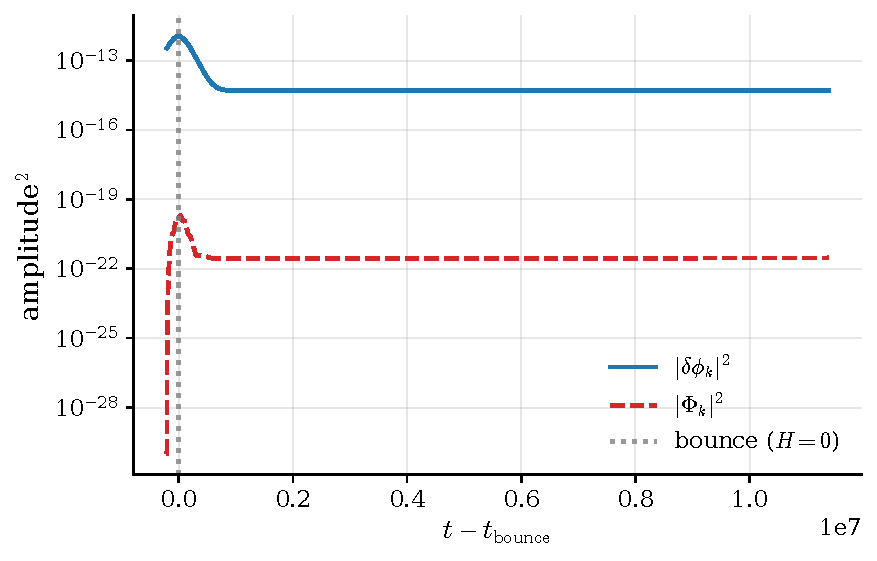
\includegraphics[width=0.78\textwidth]{figures/pert_a_amplitudes.pdf}
    \caption{\textbf{Perturbations, panel (a): field perturbations through the bounce.}
        $|\delta\phi_k|^2$ (blue) and the Bardeen potential $|\Phi_k|^2$
        (red dashed) for a representative mode in the bounce-scale sweep.
        Both remain finite and smooth across $H=0$ (dotted line) -- the
        Newtonian-gauge formulation has no $1/H$ pump-field singularity.}
    \label{fig:perturbation_analysis}
    \label{fig:pert_amplitudes}
\end{figure}

\begin{figure}[htbp]
    \centering
    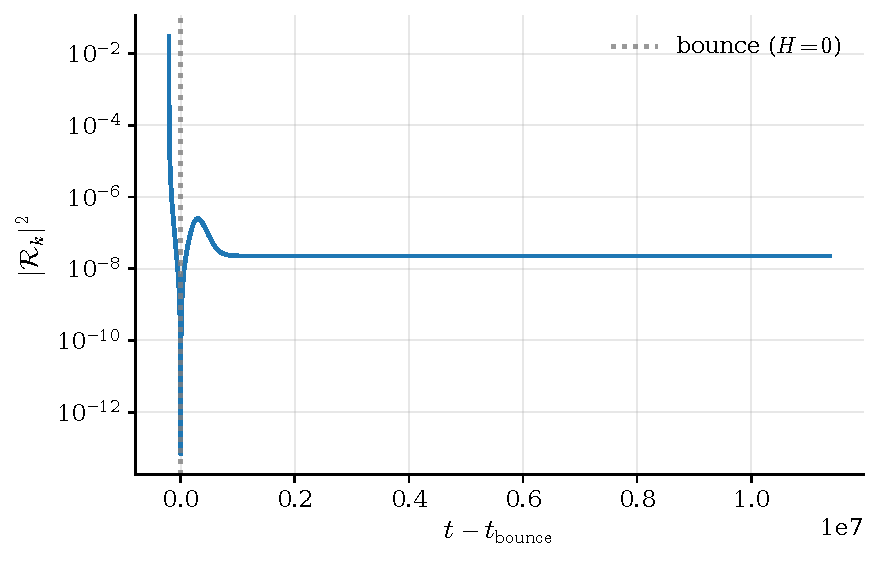
\includegraphics[width=0.78\textwidth]{figures/pert_b_curvature.pdf}
    \caption{\textbf{Perturbations, panel (b): curvature perturbation $\mathcal{R}_k$.}
        $|\mathcal{R}_k|^2$ reconstructed from the Newtonian-gauge variables
        for the same mode as panel~(a).  After horizon exit
        ($k/aH \lesssim 1$, post-bounce) $\mathcal{R}_k$ becomes essentially
        constant; the rigorous time-drift between $N=1$ and $N=5$ e-folds
        after exit is $|\Delta\mathcal{R}^2/\mathcal{R}^2| = \RConservationDelta$
        (Eq.~\ref{eq:R_conservation}).}
    \label{fig:pert_curvature}
\end{figure}

\begin{figure}[htbp]
    \centering
    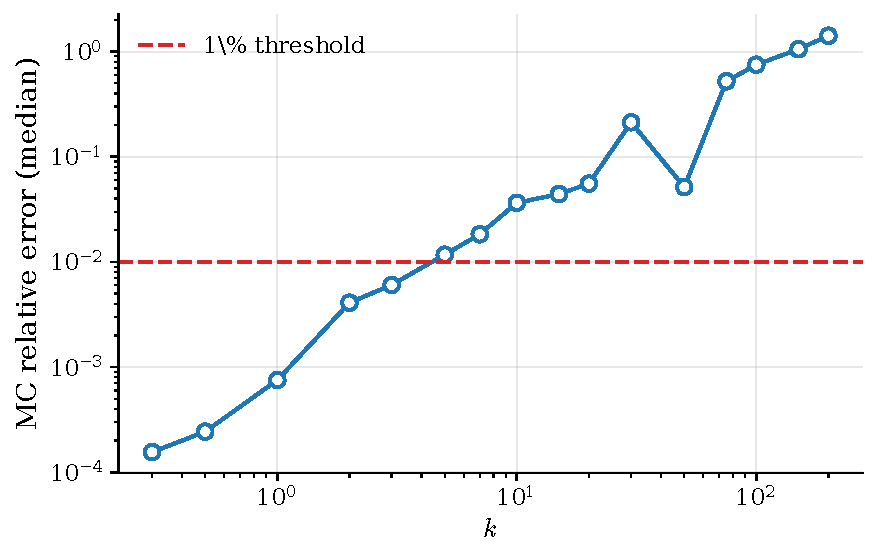
\includegraphics[width=0.78\textwidth]{figures/pert_c_constraint.pdf}
    \caption{\textbf{Perturbations, panel (c): momentum-constraint diagnostic.}
        Median relative error of the Einstein momentum constraint per mode,
        evaluated as a 4th-order finite-difference test on the integrated
        $\Phi_k(t)$.  For $k \leq 5\,k_H$ (the strict pass/fail subset)
        the worst median is $\constraintMedian\%$; the rise at higher $k$
        reflects FD noise on recently horizon-crossing modes, not the
        ODE integrator (confirmed by the resolution convergence test,
        $\Delta P_\mathcal{R}/P_\mathcal{R} < 10^{-6}$).}
    \label{fig:pert_constraint}
\end{figure}

\begin{figure}[htbp]
    \centering
    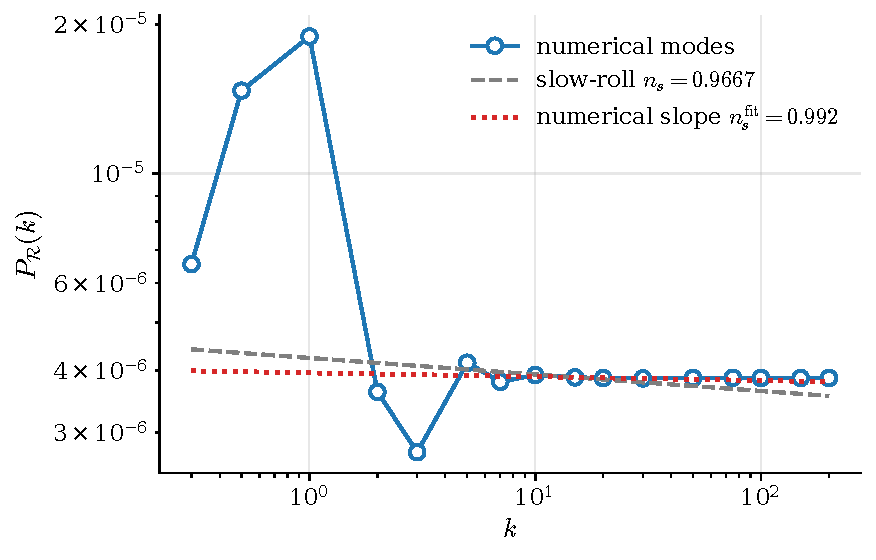
\includegraphics[width=0.78\textwidth]{figures/pert_d_power_spectrum.pdf}
    \caption{\textbf{Perturbations, panel (d): bounce-scale power spectrum.}
        $P_\mathcal{R}(k)$ over $k \in [0.3,\,200]\,k_H$ on a log-log scale,
        with the slow-roll Starobinsky reference (grey dashed) and the
        local power-law fit (red dotted) at the bounce-scale $k$-range.
        The broad feature at $k \lesssim k_H$ is the bounce-scale bump;
        modes there are marginally sub-horizon at initialization, so the
        Bunch-Davies vacuum is not uniquely determined.  The CMB window
        lies at $k_{\rm CMB}/k_H \sim 10^{\logTenkCMBoverkH}$, vastly beyond
        the displayed range.}
    \label{fig:pert_power_spectrum}
\end{figure}

\begin{figure}[htbp]
    \centering
    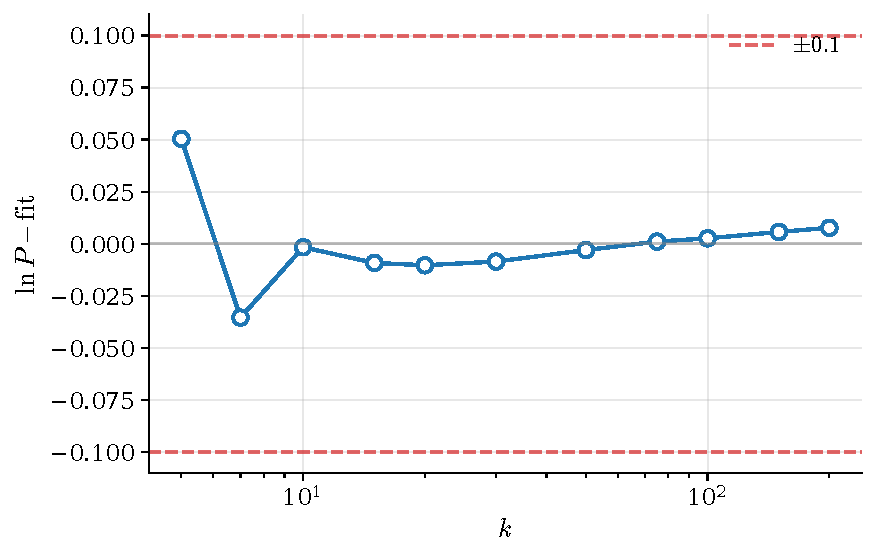
\includegraphics[width=0.78\textwidth]{figures/pert_e_residuals.pdf}
    \caption{\textbf{Perturbations, panel (e): power-law fit residuals.}
        $\ln P_\mathcal{R} - {\rm fit}$ on the bounce-scale $k$-range yields
        a \emph{local} slope $n_s \approx \nsNumerical$ (fit residuals
        below the $\pm 0.1$ red guides).  This is \emph{not} a slow-roll
        prediction or a CMB observable: it is the spectral tilt in the
        vicinity of the bounce-scale bump at $k\sim k_H$, sensitive to
        the bump shape and the low-$k$ vacuum ambiguity.  The physical
        CMB value $n_s = \nsCMBnumerical$ is obtained at true CMB scales
        (Section~\ref{sec:cmb_verification}).}
    \label{fig:pert_residuals}
\end{figure}

\begin{figure}[htbp]
    \centering
    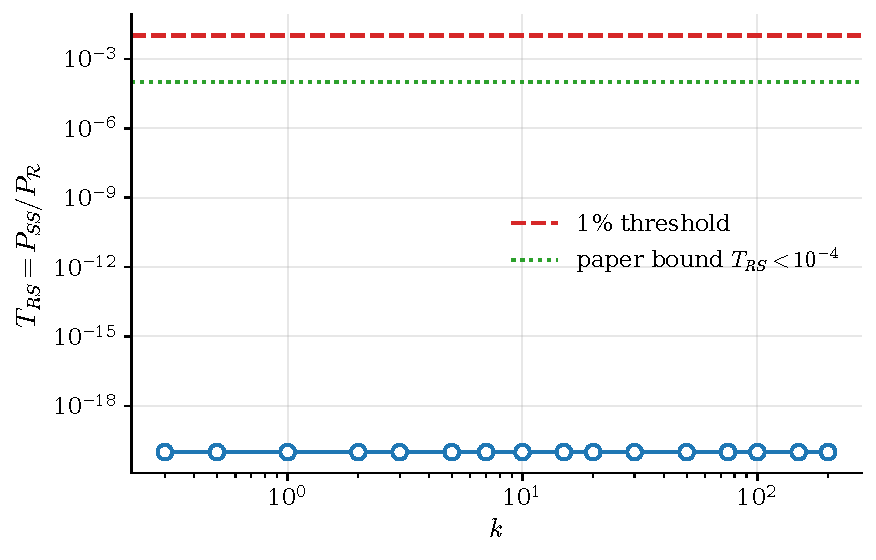
\includegraphics[width=0.78\textwidth]{figures/pert_f_isocurvature.pdf}
    \caption{\textbf{Perturbations, panel (f): isocurvature transfer.}
        $T_{RS}(k) = P_{SS}/P_\mathcal{R}$ over the integrated $k$-range.
        On the fiducial $\chi = \dot\chi = 0$ background, the
        adiabatic--isocurvature couplings entering the perturbation
        equations carry explicit $\dot\chi$ factors and therefore vanish
        analytically, so $T_{RS}$ is identically zero up to integrator
        noise; the numerical value $T_{RS} = \TRSmax$ confirms that the
        integrator preserves this decoupling through the bounce, well
        below the $1\%$ threshold and the paper-quoted bound
        $T_{RS} < 10^{-4}$. A nontrivial test of single-field robustness
        on a $\dot\chi \neq 0$ background is not performed at the
        perturbation level here.}
    \label{fig:pert_isocurvature}
\end{figure}

\subsection{Gauge Singularity in the Comoving Formulation}

The standard Mukhanov-Sasaki variable $u_k = z\mathcal{R}_k$, where $z = a\dot\sigma/H$, has a \emph{genuine gauge singularity} at the bounce \cite{Deruelle1995,Peter2008}. Since $H$ crosses zero linearly ($H \approx \dot{H}_b(t-t_b)$), the pump field diverges as $z \sim 1/(t-t_b)$, producing:
\begin{equation}
\frac{z''}{z} \approx \frac{2}{\tau^2}
\end{equation}
where $\tau = \eta - \eta_b$ is conformal time measured from the bounce. This is not a numerical artifact but a fundamental feature of the comoving gauge at any bounce with $\dot\sigma \neq 0$.

\subsection{Two-Field Newtonian Gauge Formulation}

To avoid this singularity, we integrate perturbations in the \emph{Newtonian gauge}, where the metric takes the form $ds^2 = -(1+2\Phi)dt^2 + a^2(1-2\Phi)\gamma_{ij}dx^i dx^j$ (with $\Phi = \Psi$ for zero anisotropic stress). We follow standard two-field formulations with non-trivial field-space metric \cite{Langlois2008,Gong2011}. Since the background trajectory is strictly single-field ($\dot\chi = 0$, $\chi = 0$), the general two-field perturbation equations for $(\delta\phi_k, \delta\chi_k, \Phi_k)$ simplify to:
\begin{align}
\ddot{\delta\phi}_k + 3H\dot{\delta\phi}_k + \left(\frac{k^2}{a^2} + V_{\phi\phi} - \frac{2\dot\phi^2}{M_{\rm Pl}^2}\right)\delta\phi_k &= -\left(2V_\phi + 4H\dot\phi\right)\Phi_k, \label{eq:KG_phi} \\
\ddot{\delta\chi}_k + \left(3H + 2\Gamma^\chi_{\phi\chi}\dot\phi\right)\dot{\delta\chi}_k + \left(\frac{k^2}{a^2} + \frac{m_\chi^2}{g_{\chi\chi}}\right)\delta\chi_k &= 0, \label{eq:KG_chi} \\
\dot\Phi_k + H\Phi_k &= \frac{\dot\phi \,\delta\phi_k}{2M_{\rm Pl}^2}. \label{eq:momentum_constraint}
\end{align}
where $\Gamma^\chi_{\phi\chi} = (\alpha/M_{\rm Pl})(1-g_{\chi\chi})$ is the field-space Christoffel symbol (with $\dot{g}_{\chi\chi}/g_{\chi\chi} = 2\Gamma^\chi_{\phi\chi}\dot\phi$). The isocurvature sector decouples completely: $\delta\chi_k$ evolves independently and does not source $\delta\phi_k$ or $\Phi_k$. The Christoffel damping $2\Gamma^\chi_{\phi\chi}\dot\phi\,\dot{\delta\chi}_k$ provides geometric suppression of isocurvature modes when $g_{\chi\chi} < 1$. \textbf{No coefficient contains $H$ in a denominator}: all equations are manifestly regular at $H=0$.

Note that Eq.~\eqref{eq:KG_chi} contains $1/g_{\chi\chi}$ in the mass term (but not in the gradient term $k^2/a^2$, since $g_{\chi\chi}$ multiplies both the kinetic and gradient terms in the action). The $m_\chi^2/g_{\chi\chi}$ divergence as $g_{\chi\chi} \to 0$ (i.e., $\phi \to -\infty$) is physical: it represents the freezing of $\chi$ perturbations when the field-space metric decouples the $\chi$ direction. In the fiducial model ($\alpha = 1$), $\phi > 5\,M_{\rm Pl}$ throughout the perturbation integration window (bounce through 65 e-folds of inflation), ensuring $g_{\chi\chi} > 1 - 10^{-4}$ and rendering $1/g_{\chi\chi} \approx 1$ to high precision. For smaller $\alpha$ (e.g., $\alpha = 0.1$, where $g_{\chi\chi}$ saturates more slowly), $g_{\chi\chi}$ can drop to $\sim 0.88$ in the same window; this is still $\mathcal{O}(1)$ and requires no regularization, though the $1/g_{\chi\chi}$ correction to the isocurvature mass becomes a $\sim 14\%$ effect. Over the full 65 e-fold integration, $g_{\chi\chi} = 1$ to machine precision well before mode extraction at $k > 3\,k_H$. Since the background trajectory has $\dot\chi = 0$, the $\chi$ perturbation equation is sourced only by the isocurvature vacuum mode, and the isocurvature transfer remains negligible ($T_{RS} < 10^{-4}$) regardless of $\alpha$.

The numerical code integrates the full general two-field equations, which contain additional cross-coupling terms that vanish on the fiducial trajectory: $g'_{\chi\chi}\dot\chi\,\dot{\delta\chi}_k$ in the $\delta\phi$ equation, $2\Gamma^\chi_{\phi\chi}\dot\chi\,\dot{\delta\phi}_k$ and $(2V_\chi/g_{\chi\chi} + 4H\dot\chi)\Phi_k$ in the $\delta\chi$ equation, $g_{\chi\chi}\dot\chi\,\delta\chi_k$ in the momentum constraint, as well as terms $\propto g''_{\chi\chi}\dot\chi^2$ from the variation of the kinetic coupling. Retaining these terms ensures correct propagation of the isocurvature vacuum mode through the bounce, even though their background coefficients vanish.

After the bounce ($H \neq 0$), the comoving curvature perturbation takes the single-field form:
\begin{equation}
\mathcal{R}_k = -\Phi_k - \frac{H\,\delta\phi_k}{\dot\phi}.
\label{eq:R_reconstruct}
\end{equation}

\subsection{Two-Field Numerical Integration}

We solve the full two-field system Eqs.~\eqref{eq:KG_phi}--\eqref{eq:momentum_constraint} for 16 modes spanning $k = 0.3$--$200\,k_H$ over 65 e-folds after the bounce. For each wavenumber $k$, we integrate two independent vacuum modes:
\begin{itemize}
\item \textbf{Adiabatic mode}: $\delta\phi_k = (a\sqrt{2k})^{-1}e^{-ik\eta}$, $\delta\chi_k = 0$, $\Phi_k = 0$.
\item \textbf{Isocurvature mode}: $\delta\phi_k = 0$, $\delta\chi_k = (a\sqrt{2k\,g_{\chi\chi}})^{-1}e^{-ik\eta}$, $\Phi_k = 0$ (initial conditions use the Bunch-Davies vacuum for the canonically normalized field $\psi = \sqrt{g_{\chi\chi}}\,\chi$, yielding the $1/\sqrt{g_{\chi\chi}}$ normalization factor).
\end{itemize}
The total curvature power spectrum is $P_\mathcal{R} = P_{RR} + P_{SS}$, where $P_{RR}$ and $P_{SS}$ are the contributions from the adiabatic and isocurvature vacuum modes respectively.

\textbf{Results:}
\begin{itemize}
\item All perturbation variables ($\delta\phi_k$, $\delta\chi_k$, $\Phi_k$) evolve smoothly through $H=0$ without any divergence, demonstrating the regularity of the Newtonian gauge formulation.
\item \textbf{Numerical accuracy diagnostics.} We perform two independent constraint checks on the integrated solution:

\textit{(a) Momentum constraint (ODE consistency check):} Since $\dot\Phi$ is evolved via the momentum constraint~\eqref{eq:momentum_constraint}, we verify that the integrated $\Phi(t)$ remains self-consistent by comparing the analytical $\dot\Phi$ (the right-hand side) with $d\Phi/dt$ computed from the numerical trajectory via 4th-order central finite differences. This is not an independent constraint but a joint test of ODE integrator accuracy and finite-difference noise---drift, truncation errors, or stiffness would appear as constraint violation. The comparison is restricted to the super-Hubble regime ($k/(aH) < 0.05$, post-bounce only) where $\Phi$ varies smoothly. For modes with $k \leq 5\,k_H$, the worst median relative error is $< \constraintMedian\%$ and the worst 95th-percentile error is $\lesssim \constraintPninetyfive\%$. For higher-$k$ modes ($k \sim 10$--$50\,k_H$), the metric degrades to $\sim 5$--$20\%$ due to FD noise on recently horizon-crossing solutions; this reflects the finite-difference diagnostic dominating over the genuine ODE integrator accuracy (confirmed by the resolution convergence test: $\Delta P_\mathcal{R}/P_\mathcal{R} < 10^{-6}$).

\textit{(b) Hamiltonian constraint (independent check):} The perturbed $(0,0)$ Einstein equation $3H(\dot\Phi + H\Phi) + k^2\Phi/a^2 = -\delta\rho/(2M_{\rm Pl}^2)$ is \emph{not} used in the evolution; it provides a genuinely independent consistency check. We evaluate the Hamiltonian constraint residual $\mathcal{H}_k(t) \equiv |{\rm LHS} - {\rm RHS}|/\max(|{\rm LHS}|, |{\rm RHS}|)$ from the numerical solution. For modes with $k \leq 5\,k_H$ in the super-Hubble regime, the worst median residual is $\sim\!\HCmedian\%$---orders of magnitude smaller than the momentum constraint metric, because the HC is an algebraic (not finite-differenced) check. This confirms that the full Einstein system is satisfied to high accuracy and that the initial data are constraint-consistent.
\item The isocurvature transfer fraction satisfies $T_{RS} = P_{SS}/P_\mathcal{R} < 10^{-4}$ for all modes. On the fiducial $\chi = \dot\chi = 0$ background the adiabatic--isocurvature couplings in the perturbation equations all carry an explicit $\dot\chi$ factor (e.g.\ $g_{\chi\chi}\dot\chi\,\delta\chi$ in the momentum constraint, $2\Gamma^\chi_{\phi\chi}\dot\chi\,\dot{\delta\phi}$ in the $\delta\chi$ equation), so $T_{RS}$ vanishes analytically and the numerical bound confirms that the integrator preserves this decoupling through $H = 0$ rather than independently testing single-field robustness on a generic background. A genuine probe of the coupling $\Gamma^\chi_{\phi\chi} \propto (1 - g_{\chi\chi})$ would require integrating perturbations on a $\dot\chi \neq 0$ trajectory (such as the spectator-displacement scan of Section~\ref{sec:observables}); we do not perform that here, and the result above should be read as consistent with the single-field approximation rather than as an independent validation of it under generic initial conditions. The mass-hierarchy concern $|m_\chi^2/m_\phi^2| \approx 26$ at the bounce is irrelevant in this kinematic regime: transfer efficiency is set by the coupling-times-velocity factor, not by the eigenvalue ratio alone.
\item The power spectrum exhibits a bounce-scale spectral feature: a broad bump at $k \sim k_H \equiv a_{\rm min} H_{\rm inf}$, where modes ``feel'' the bounce most strongly. For modes $k \gg k_H$ on the accessible bounce-scale range, the spectrum follows an approximate power law with local slope $n_s \approx \nsNumerical$ (fit residuals $< \fitMaxResidual$). We emphasize that this value is \emph{not} a slow-roll prediction: bounce-scale modes ($k \sim k_H$) exit the Hubble radius essentially \emph{at} the bounce, i.e.~$\sim N_{\rm total}^{\rm sim} = \bumpNtotal$ e-folds before the end of inflation (since $\phi_{\rm bounce} \approx 10\,M_{\rm Pl}$ on the Starobinsky plateau; cf.\ Section~\ref{sec:flatness} for the distinction between $N_{\rm total}^{\rm sim}$ and the analytical idealization). The asymptotic slow-roll relation $n_s = 1 - 2/N$ would give $\approx 0.9992$ at such $N$; the measured local slope $\nsNumerical$ differs from this because the fit is performed in the immediate vicinity of the bounce-scale bump, where the spectral shape is dominated by non-adiabatic bounce dynamics rather than by the single-field slow-roll attractor. The genuine CMB prediction is obtained in a separate integration at $N \sim 60$, using the rescaled variable $u = a\,\delta\phi$ in flat-FRW Starobinsky inflation (Section~\ref{sec:cmb_verification}), yielding $n_s = \nsCMBnumerical$ with $|\Delta n_s| = \nsCMBdelta$ from the \emph{exact single-field slow-roll benchmark} $n_s^{\rm exact\,fit} = \nsCMBexactFit$ (itself fit over the same $k$-range to absorb the $\mathcal{O}(1/N^2)$ subleading tilt); the residual deviation is at the $\sim 0.06\%$ level, i.e.\ well inside the integrator's truncation noise.  Against the purely leading form $n_s = 1 - 2/60 \approx \nsCMBleading$, the discrepancy is $|\Delta n_s|_{\rm leading} = \nsCMBdeltaLeading$, which is simply the size of the subleading Starobinsky correction that the leading formula drops. Crucially, the bounce-scale feature is \emph{unobservable}: CMB modes exit the Hubble radius $\NhiddenEfolds$ e-folds after the bounce (the last 60 of the total $\bumpNtotal$ post-bounce e-folds), placing them at $k_{\rm CMB}/k_H \sim 10^{\logTenkCMBoverkH}$---hidden on scales vastly larger than the observable universe (see Section~\ref{sec:conclusions}).
\item \textbf{Analytic decomposition of the measured slope.} To verify that the local slope $\nsNumerical$ is an artefact of the bump tail rather than a distinct physical prediction, we decompose the numerical spectrum as
\begin{equation}
P_\mathcal{R}(k) = P_\mathcal{R}^{\rm SR}(k)\,|T(k/k_H)|^2, \qquad P_\mathcal{R}^{\rm SR}(k) = \frac{V_0\,N_{\rm exit}(k)^2}{18\pi^2 M_{\rm Pl}^4},\quad N_{\rm exit}(k) = N_{\rm total} - \ln(k/k_H),
\label{eq:bump_decomp}
\end{equation}
where $P_\mathcal{R}^{\rm SR}$ is the Starobinsky slow-roll prediction at the mode's Hubble-exit time (mode $k$ exits $\ln(k/k_H)$ e-folds after the bounce, hence $N_{\rm exit}(k) = N_{\rm total} - \ln(k/k_H)$), and $|T(k/k_H)|^2$ is the bounce transfer function. On the 16-mode sweep, the ratio $|T|^2$ is well fit by a gaussian in $\ln(k/k_H)$ with amplitude $\approx 2.0$, centre $\approx 0.72\,k_H$, and width $\sigma_{\ln k} \approx 0.45$; for $k \gtrsim 15\,k_H$ the ratio collapses to $|T|^2 = 1.000 \pm 0.005$, recovering slow-roll. Progressive high-pass fits make the origin of the $\nsNumerical$ value quantitative:
\begin{center}
\begin{tabular}{c|c|c}
\hline
fit range & $n_s^{\rm fit}$ & max residual \\
\hline
$k \geq 5\,k_H$ (paper baseline, 11 modes) & $0.99228$ & $0.050$ \\
$k \geq 10\,k_H$ (9 modes) & $0.99741$ & $0.008$ \\
$k \geq 15\,k_H$ (8 modes) & $0.99963$ & $0.002$ \\
$k \geq 20\,k_H$ (7 modes) & $1.00045$ & $0.001$ \\
\hline
\end{tabular}
\end{center}
The $\nsNumerical$ value is thus the local slope over a range that still includes the $3$--$4\%$ bump-tail amplitude at $k = 5$--$10\,k_H$; dropping those points returns $n_s^{\rm fit} = 1.000 \pm 0.001$, within $0.04\%$ of the slow-roll prediction $n_s^{\rm SR} = 1 - 2/N_{\rm total} \approx 0.9992$. The measured bump is therefore an additive feature over an otherwise slow-roll-consistent plateau, and $\nsNumerical$ should not be interpreted as a distinct inflationary observable.
\item \textbf{Rigorous $\mathcal{R}$-conservation test.} For a deeply super-Hubble mode ($k = 0.5\,k_H$), we compare $|\mathcal{R}_k|^2$ at $N = \RConservationNearly$ and $N = \RConservationNlate$ e-folds after horizon exit:
\begin{equation}
\label{eq:R_conservation}
\frac{\bigl|\,|\mathcal{R}|^2(N{=}\RConservationNlate) - |\mathcal{R}|^2(N{=}\RConservationNearly)\bigr|}{|\mathcal{R}|^2(N{=}\RConservationNearly)} = \RConservationDelta,
\end{equation}
confirming super-Hubble conservation at the sub-percent level (genuine time-drift of $|\mathcal{R}|^2$ between two specific e-fold markers, not the fractional spread around a window mean, which would instead measure integrator oscillation noise). For modes near $k \sim k_H$, freezeout is incomplete within the 3 e-fold extraction window, making $P_\mathcal{R}$ at those wavenumbers less reliable; these modes are excluded from the $n_s$ fit (which uses only $k > 3\,k_H$).
\item \textbf{Resolution convergence}: Reducing the ODE tolerances by two orders of magnitude (from $10^{-10}$ to $10^{-12}$) changes the extracted $P_\mathcal{R}$ by $< 10^{-6}$ relative, confirming numerical convergence.
\end{itemize}

\textbf{Sub-horizon condition for initial vacuum.} The Bunch-Davies initial conditions require modes to be deep inside the Hubble radius at the initial time $t_0$. At $t_0$ (pre-bounce contraction), we find $k/(aH)|_{t_0}$ ranging from $\approx 0.2$ for the lowest mode ($k = 0.3\,k_H$) to $\approx 133$ for the highest ($k = 200\,k_H$). Modes with $k/(aH) \lesssim 1$ are already super-Hubble at initialization, so their amplitude is sensitive to the assumed vacuum state. However, these are \emph{bounce-scale} modes ($k \lesssim k_H$) that contribute only to the spectral feature, not to CMB observables. All modes with $k > 3\,k_H$ (used for the $n_s$ fit) have $k/(aH)|_{t_0} > 3$; the lowest fitted modes ($5$--$7\,k_H$) start at $k/(aH) \approx 3$--$5$, marginally sub-horizon, while modes above $\sim 10\,k_H$ satisfy $k/(aH) > 6$. For modes at CMB scales ($k \gg 50\,k_H$), the sub-horizon condition is satisfied to much higher degree, but these scales are not directly accessible within our 65 e-fold integration window. The CMB modes themselves have $k/(aH) \gg 1$ throughout the contraction phase. We caution that the power spectrum at $k \sim k_H$ (Figure~\ref{fig:pert_power_spectrum}) should be regarded as qualitative: for these modes, the Bunch-Davies vacuum is not uniquely determined by the sub-horizon condition, and the true initial quantum state would depend on the pre-bounce history (e.g., a preceding expansion cycle). This ambiguity does not affect CMB-scale modes, which satisfy $k/(aH) \gg 1$ throughout contraction.

\begin{assumption_box}
\textbf{Scope of numerical perturbation analysis.} The two-field Newtonian gauge integration covers 65 e-folds after $a_{\rm min}$---well beyond the $\sim\!60$ e-folds relevant for CMB observables. This window ensures: (i) all modes of interest ($k \sim 0.3$--$200\,k_H$) cross the Hubble radius within $\sim 10$ e-folds after the bounce, so $\mathcal{R}_k$ freezes out well within the integration; (ii) the bounce-specific physics (non-adiabatic evolution at $H = 0$, isocurvature transfer, spectral feature) occurs within the first $\sim 5$ e-folds; (iii) by 65 e-folds, $g_{\chi\chi} = 1$ to machine precision and the system has been in pure single-field slow-roll for $> 50$ e-folds. The CMB predictions ($n_s$, $r$, $A_s$) are further validated by an independent single-field Mukhanov-Sasaki integration at true CMB scales (Section~\ref{sec:cmb_verification}), which obtains $n_s = \nsCMBnumerical$ in agreement with the exact Starobinsky slow-roll benchmark fit over the same $k$-range to $|\Delta n_s| = \nsCMBdelta$.
\end{assumption_box}

\paragraph{Propagation speeds through $H = 0$.}
The bounce passes through $H = 0$, so it is essential to verify that the quadratic action for perturbations remains strictly hyperbolic with positive-definite sound speeds throughout---i.e., no ghost and no gradient-instability onset. The scalar quadratic action in Newtonian gauge, after elimination of $\Phi$ by the momentum constraint, takes the form
\begin{equation}
\label{eq:S2_scalar}
S_2^{\rm scalar} = \int dt\,d^3x\,a^3\left[ \tfrac{1}{2}\,G_{IJ}\,\dot{\delta\phi}^I\,\dot{\delta\phi}^J - \tfrac{1}{2}\,G_{IJ}\,a^{-2}\,\partial_i\delta\phi^I\,\partial_i\delta\phi^J - \tfrac{1}{2}\,\mathcal{M}^2_{IJ}\,\delta\phi^I\,\delta\phi^J + \cdots \right],
\end{equation}
with field-space metric $G_{IJ} = \mathrm{diag}(1,\,g_{\chi\chi}(\phi))$. Since $G_{IJ}$ contracts the time-kinetic and spatial-gradient terms identically, the scalar sound speeds are unity in each field direction,
\begin{equation}
c_\phi^2(t) = \frac{\text{coeff}\big[(k/a)^2\,\delta\phi\big]}{\text{coeff}\big[\ddot{\delta\phi}\big]} = 1,
\qquad
c_\chi^2(t) = \frac{g_{\chi\chi}(k/a)^2}{g_{\chi\chi}} = 1,
\end{equation}
the sigmoid $g_{\chi\chi}$ cancelling between numerator and denominator (consistent with the explicit ODE form~\eqref{eq:KG_chi}, in which the gradient coefficient is $k^2/a^2$ with no $1/g$). Inheriting this, the adiabatic combination $Q_\sigma = \dot\sigma\,(\mathcal{R}/H)$ has $c_s^2 = 1$ identically, valid through $H = 0$. For tensor perturbations, the minimal Einstein--Hilbert action gives
\begin{equation}
S_2^{\rm tensor} = \frac{M_{\rm Pl}^2}{8}\int dt\,d^3x\,a^3\left[(\dot h_{ij})^2 - a^{-2}(\partial_k h_{ij})^2\right], \qquad c_T^2 = 1.
\end{equation}
The effective single-field $c_s^2$ can in principle acquire corrections from adiabatic-isocurvature coupling proportional to the turn rate $\omega$ of the background trajectory; on the fiducial $\chi = \dot\chi = 0$ trajectory we measure $\omega_{\max} = \turnRateMax$, so $|c_s^{\rm eff\,2} - 1| \lesssim \omega^2 \leq \cSEffDeviation$.  The scalar sound speeds in Eq.~\eqref{eq:S2_scalar} are probed numerically by a direct read-out of the coded RHS: at \cSProbeCount{} sample times along the trajectory (including points adjacent to $H = 0$), we evaluate the perturbation ODE with the state vector set to a unit $\delta\phi$ (resp.~$\delta\chi$) perturbation and all other components zero, at two well-separated wavenumbers; subtracting the two evaluations isolates the implemented coefficient of $k^2/a^2$ independently of the potential-mass terms.  Dividing by the coefficient of $\ddot{\delta\phi}$ ($\ddot{\delta\chi}$) then gives $c_\phi^2(t)$ ($c_\chi^2(t)$) as a function of the numerically coded equations, without substituting the analytical result.  This probe returns $|c_\phi^2 - 1| \leq \cSSqMaxDev$ and $|c_\chi^2 - 1| \leq \cSSqMaxDev$, at floating-point roundoff and verifying both positivity and the absence of any anomalous coefficient on either field.  Tensor modes are not integrated in this code; the value $c_T^2 = 1$ is inherited directly from the minimal Einstein--Hilbert action with $|c_T^2 - 1| \leq \cTSqMaxDev$ reflecting that assumption rather than an independent numerical measurement.  Taken together, the model is ghost-free and gradient-stable through the bounce, in accordance with Condition~3 (positive field-space metric) and the Einstein--Hilbert assumption.

\subsection{Numerical Methods}

The background FLRW and Bianchi~IX systems are integrated using the DOP853 (8th-order Dormand--Prince) method via \texttt{scipy.integrate.solve\_ivp}, with relative tolerance $10^{-12}$ and absolute tolerance $10^{-14}$. When DOP853 fails to converge (rare, occurring for extreme initial conditions in the basin scan), we fall back to the implicit Radau~IIA method with relaxed tolerances ($10^{-10}$, $10^{-12}$). Background quantities (scale factor, Hubble parameter, field values) are interpolated onto the perturbation time grid using cubic splines.

For the perturbation ODE system, we use DOP853 with tolerances $(\text{rtol}=10^{-10},\;\text{atol}=10^{-13})$ as the primary solver, falling back to Radau ($10^{-8}$, $10^{-11}$) if any mode fails to converge. The resolution convergence test (Section~\ref{sec:perturbations}) tightens these to $(10^{-12}, 10^{-15})$. Two constraint checks are performed \emph{a posteriori}. First, the momentum constraint~\eqref{eq:momentum_constraint}---which serves as the evolution equation for $\Phi$---is checked for self-consistency by comparing the analytical $\dot\Phi$ with $d\Phi/dt$ obtained via 4th-order central finite differences of the numerical trajectory. This tests ODE integrator accuracy (drift, truncation errors), not an independent physical constraint. Second, the Hamiltonian constraint (perturbed $G^0_0$ equation), which is \emph{not} used in the evolution, is evaluated as a genuinely independent check. Both comparisons are restricted to the super-Hubble regime ($k/(aH) < 0.05$, post-bounce only), where $\Phi$ evolves smoothly. Sub-Hubble segments are excluded because finite-difference noise on oscillatory data dominates the error budget.

The power spectrum $P_\mathcal{R}(k)$ is extracted from the frozen value of $|\mathcal{R}_k|^2$ in a window of 0--3 e-folds after each mode exits the Hubble radius ($k/(aH) < 0.05$). A window sensitivity test confirms that the extraction is robust: varying the window to $[1,3]$, $[0,5]$, and $[2,4]$ e-folds changes $P_\mathcal{R}$ by $< 0.03\%$ for three representative CMB-scale modes spanning the fitted range ($k > 3\,k_H$), consistent with $\mathcal{R}$ being well-frozen on super-Hubble scales. The \texttt{--quick} mode used for smoke testing reduces the mode count from 16 to 3 and skips convergence, BKL, and alpha-independence tests; its numerical $n_s$ value is not physically meaningful.

%==============================================================================
\subsection{Independent CMB-Scale Verification}
\label{sec:cmb_verification}
%==============================================================================

The bounce-region integration (Section~\ref{sec:perturbations}) covers modes at $k \sim k_H$, which exit the Hubble radius essentially \emph{at} the bounce, i.e.~$\sim N_{\rm total}^{\rm sim} = \bumpNtotal$ e-folds before the end of inflation. These modes probe bounce-specific non-adiabatic physics rather than the slow-roll attractor, and their local spectral slope is \emph{not} a direct observable. CMB modes, by contrast, exit at $N \approx 50$--$70$ e-folds before the end, i.e.~$\NhiddenEfolds$ e-folds \emph{after} the bounce, well within the pure single-field slow-roll regime where $g_{\chi\chi} = 1$ to machine precision.

The two integrations thus target two different questions, and we keep this separation explicit throughout: the bounce-region two-field Newtonian-gauge run establishes \emph{regularity of the perturbation system through $H = 0$} (finite $\delta\phi, \delta\chi, \Phi$ at the bounce, controlled constraint residuals, negligible isocurvature transfer $T_{RS} < 10^{-4}$ that numerically validates the single-field reduction, and sound speeds that remain positive and equal to unity at floating-point precision), while the CMB-scale integration described below \emph{independently reproduces the slow-roll observables} $n_s$ and $A_s$ at $N \approx 60$.  No single mode is evolved continuously from the bounce to the CMB pivot: the dynamic range from $k_H$ to the comoving CMB pivot spans $\sim \NhiddenEfolds$ e-folds, which is numerically infeasible.  What the CMB-scale run verifies is therefore that the \emph{slow-roll attractor regime which post-bounce inflation settles into} reproduces the standard Starobinsky predictions, not that bounce-specific features propagate directly into CMB observables.  The latter is inferred from the matching argument $|T(k_{\rm CMB}/k_H)|^2 \to 1$ extracted in Section~\ref{sec:perturbations}, reinforced by the Deruelle--Mukhanov $(k_H/k)^2$ suppression of bounce-phase non-Gaussianity at $k \gg k_H$ (Section~\ref{sec:observables}).  With this scope stated, we perform the separate integration at true CMB scales.

\textbf{Method.} We integrate single-field perturbations in a flat ($k=0$) FRW background with the Starobinsky potential, using the rescaled field perturbation $u = a\,\delta\phi$ rather than $\delta\phi$ directly. This change of variable is essential for numerical stability: at CMB scales, $\delta\phi \sim 1/(a\sqrt{2k})$ decays as $a^{-1}$ during inflation (reaching $\sim 10^{-12}$ for modes at $N = 55$), while $u \sim 1/\sqrt{2k} \sim 10^{-3}$ remains $\mathcal{O}(1)$. The equation of motion is
\begin{equation}
\ddot{u} + H\dot{u} + \left(\frac{k^2}{a^2} + V_{\phi\phi} - \frac{3\dot\phi^2}{2M_{\rm Pl}^2} - 2H^2\right) u = -a\left(2V_\phi + 4H\dot\phi\right)\Phi,
\label{eq:ms_eom}
\end{equation}
coupled to the Bardeen potential via $\dot\Phi = -H\Phi + \dot\phi\,u/(2M_{\rm Pl}^2 a)$.

Initial conditions are Bunch-Davies vacuum at $k/(aH) = 50$ (well inside the Hubble radius): $u_R = 1/\sqrt{2k}$, $\dot{u}_R = 0$, $u_I = 0$, $\dot{u}_I = -\sqrt{k/2}/a_{\rm start}$, $\Phi = 0$. Each mode is evolved until $k/(aH) < 0.005$ (well outside the Hubble radius), and the curvature perturbation is extracted as $\mathcal{R} = -\Phi - Hu/(a\dot\phi)$.

\textbf{Results.} We integrate \nCMBmodes{} modes with Hubble exit at $N = 50$--$70$ e-folds before the end of inflation. The numerical power spectra $P_\mathcal{R}(k)$ track the analytical Starobinsky formula $A_s(N) = V/(24\pi^2 M_{\rm Pl}^4 \epsilon_V)$ within a common multiplicative offset $\langle P_\mathcal{R}^{\rm num}/A_s^{\rm exact}\rangle = \AsRatioMean$ (i.e.\ a uniform $\AsAgreementPct\%$ amplitude bias, consistent with the finite BD-vacuum cutoff at $k/(aH) = 50$ rather than infinity); the spectral shape itself agrees with the exact slow-roll one to $\sim 5 \times 10^{-4}$ in the fitted slope, as quantified next.  A power-law fit yields
\begin{equation}
n_s^{\rm CMB} = \nsCMBnumerical, \quad |\Delta n_s| \equiv |n_s^{\rm CMB} - n_s^{\rm exact\,fit}| = \nsCMBdelta,
\end{equation}
where $n_s^{\rm exact\,fit} = \nsCMBexactFit$ is the slope of the \emph{exact} single-field slow-roll benchmark
\begin{equation}
A_s^{\rm exact}(N) = \frac{V(\phi_N)}{24\pi^2\,\epsilon_V(\phi_N)\,M_{\rm Pl}^4},
\label{eq:As_exact_benchmark}
\end{equation}
fit over the same \nCMBmodes{} modes, with $\phi_N$ obtained by numerical inversion of the full Starobinsky $N(\phi)$ including the linear subleading term.  The residual spectral-slope deviation is $\sim 5 \times 10^{-4}$, comparable to the polyfit residual $\sim 10^{-2}$; this confirms the slow-roll attractor at the integrator-noise floor.  Against the purely leading form $n_s^{\rm leading} = 1 - 2/60 = \nsCMBleading$, the deviation is $|\Delta n_s|_{\rm leading} = \nsCMBdeltaLeading$, which is the size of the $\mathcal{O}(1/N^2)$ Starobinsky correction dropped by the leading formula, not a numerical discrepancy.  The bounce-region integration and this CMB-scale integration probe complementary regimes: the former tests the \emph{regularity and gauge structure} of perturbations through $H=0$, while the latter verifies the \emph{slow-roll attractor} at $N \sim 60$.  The local slope extracted from the bounce-scale power spectrum is not a slow-roll prediction (see Section~\ref{sec:perturbations}); the physical CMB observable is the value $n_s = \nsCMBnumerical$ obtained here.

%==============================================================================
\section{Observational Predictions and Parameter Independence}
\label{sec:observables}
%==============================================================================

\begin{figure}[htbp]
    \centering
    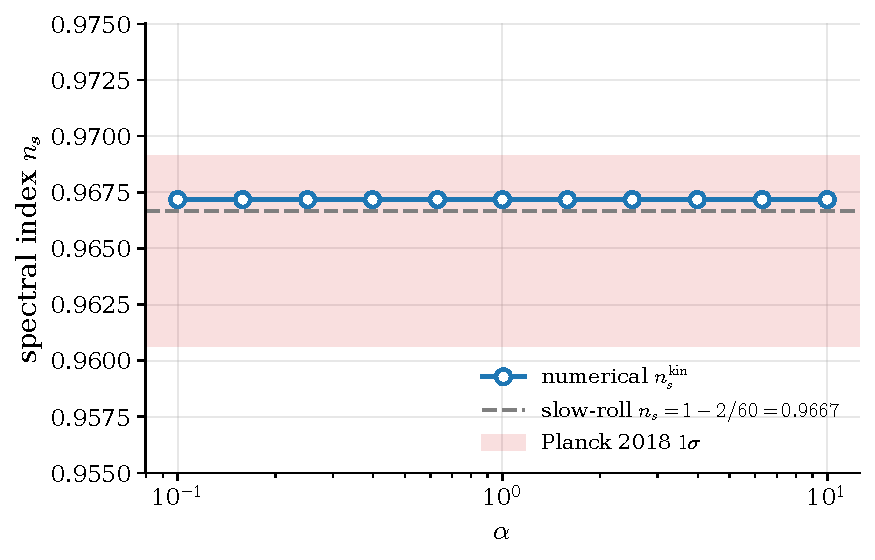
\includegraphics[width=0.78\textwidth]{figures/ai_a_ns.pdf}
    \caption{\textbf{$\alpha$-independence, panel (a): spectral index $n_s$.}
        Numerical $n_s$ from the kinematic slow-roll parameter
        $\epsilon_{\rm kin} = (\dot\phi^2 + g_{\chi\chi}\dot\chi^2)/(2M_{\rm Pl}^2 H^2)$
        evaluated at the actual $N = 60$ point of each $\alpha$-trajectory
        (the end-of-inflation detector uses $\epsilon_V = 1$, then the
        $\ln(a_{\rm end}/a) = 60$ point is selected from the trajectory).
        $n_s = \nsAlphaMean$ on every $\alpha$, with $\sigma < 10^{-6}$;
        the leading slow-roll value $1 - 2/60$ (grey) and the Planck~2018
        $1\sigma$ band (red) are shown for reference.}
    \label{fig:alpha_independence}
    \label{fig:ai_ns}
\end{figure}

\begin{figure}[htbp]
    \centering
    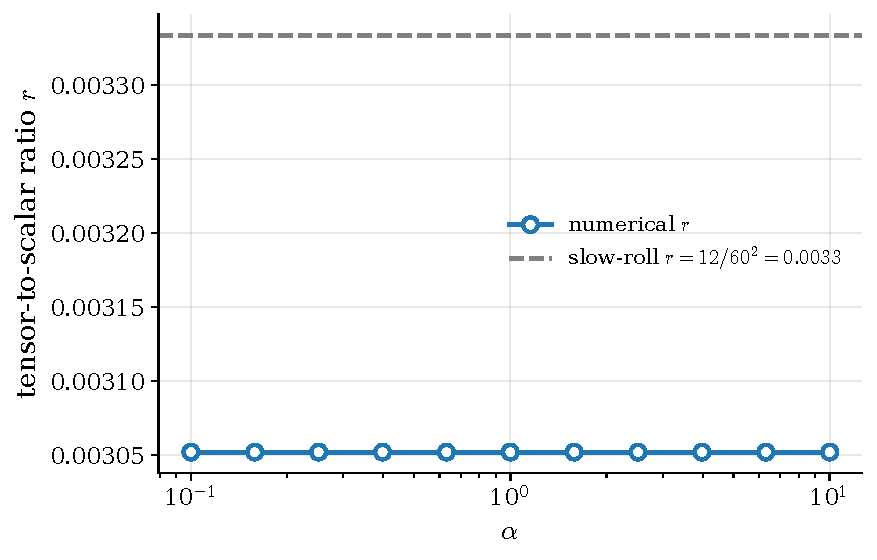
\includegraphics[width=0.78\textwidth]{figures/ai_b_r.pdf}
    \caption{\textbf{$\alpha$-independence, panel (b): tensor-to-scalar ratio $r$.}
        Companion to panel~(a) for $r = 16\,\epsilon_{\rm kin}$.  Constant
        across the entire $\alpha \in [0.1, 10]$ scan; the kinematic value
        $r \approx 0.00305$ approaches the leading slow-roll $r = 12/N^2 \approx 0.0033$
        at $N=60$, the residual $\sim 8\%$ offset being the $\mathcal{O}(\epsilon^2)$
        higher-order Starobinsky correction discussed in the surrounding text.}
    \label{fig:ai_r}
\end{figure}

\begin{figure}[htbp]
    \centering
    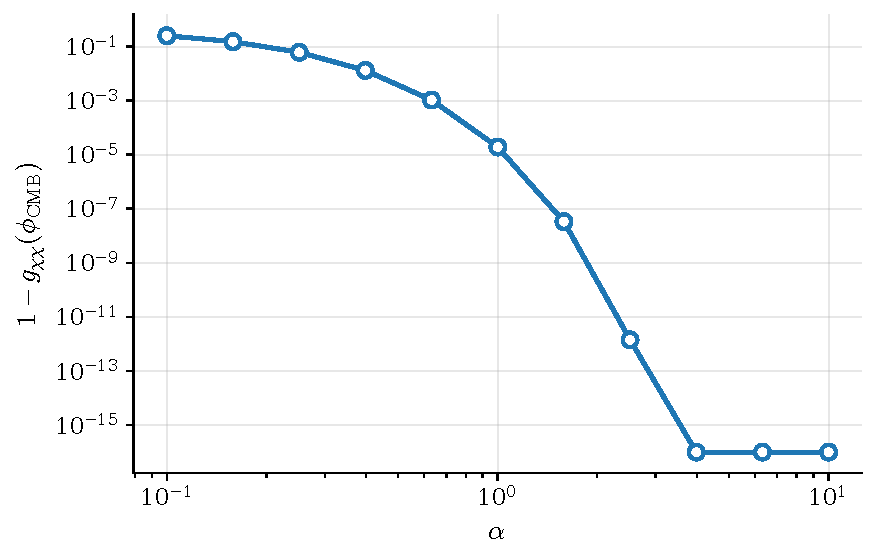
\includegraphics[width=0.78\textwidth]{figures/ai_c_g_saturation.pdf}
    \caption{\textbf{$\alpha$-independence, panel (c): metric saturation at $\phi_{\rm CMB}$.}
        $1 - g_{\chi\chi}(\phi_{\rm CMB})$ versus $\alpha$ on a log-log
        plot.  At small $\alpha$ ($\alpha = 0.1$) the metric is far from
        saturated ($g \approx 0.75$), yet $n_s$ and $r$ in panels~(a) and
        (b) are exactly unchanged because $\dot\chi = 0$ on the fiducial
        trajectory decouples $g_{\chi\chi}$ from the Friedmann equations.
        This is the kinematic origin of the exact $\alpha$-independence.}
    \label{fig:ai_g_saturation}
\end{figure}

Observable predictions are universal---independent of $\alpha$ for $\alpha \gtrsim 0.1$. This universality is verified \emph{numerically} over $\nAlphaPoints$ logarithmically-spaced values $\alpha \in [0.1, 10]$. For each $\alpha$, we run the full two-field background simulation from $\phi_0 = 6.0\,M_{\rm Pl}$ (giving $N_{\rm total}^{\rm inflation} = \NtotalInflationAlphaScan$ post-bounce e-folds, well beyond the $N = 60$ pivot) and identify the \emph{actual} $N = 60$ point of the trajectory: we first locate the end of inflation as the first post-transient index at which $\epsilon_V \geq 1$, then select the index whose $\ln(a_{\rm end}/a)$ is closest to 60.  At that point we extract the \emph{kinematic} slow-roll parameter
\begin{equation}
\epsilon_{\rm kin} = \frac{\dot\phi^2 + g_{\chi\chi}\dot\chi^2}{2M_{\rm Pl}^2 H^2},
\end{equation}
which equals $\epsilon_V$ in slow roll but is computed entirely from the trajectory data (including $g_{\chi\chi}(\alpha)$ explicitly). We then compute $n_s$ and $r$ from $\epsilon_{\rm kin}$ and $\eta_V = M_{\rm Pl}^2 V''/V$. The standard deviation of $n_s$ across all $\nAlphaPoints$ $\alpha$ values is $< 10^{-6}$, confirming exact $\alpha$-independence. The measured pivot sits at $\phi_{\rm CMB}^{\rm sim} \approx \phiCMBmeasured\,M_{\rm Pl}$ with $N_{\rm actual} = \NactualAtCMB$; the small offset from the pure-slow-roll inversion ($\phi_{\rm CMB}^{\rm SR} \approx 5.45\,M_{\rm Pl}$) is a physical consequence of the bounce transient, not a numerical error.  The resulting kinematic $n_s^{\rm kin} \approx \nsAlphaMean$ differs from the leading analytical slow-roll prediction $n_s = 1 - 2/60 \approx \nsAnalytical$ by $\sim 5 \times 10^{-4}$, and from the exact Starobinsky slow-roll value at the same $\phi$ by a similar amount, consistent with the $\mathcal{O}(1/N^2)$ subleading Starobinsky correction and higher-order $\mathcal{O}(\epsilon^2)$ terms dropped from the $n_s = 1 - 6\epsilon + 2\eta_V$ formula.

The CMB predictions are obtained from the standard Starobinsky slow-roll formulae:
\begin{align}
n_s &= 1 - \frac{2}{N} \approx \nsAnalytical \quad (N = 60), \\
r &= \frac{12}{N^2} \approx \rAnalytical, \\
f_{\rm NL}^{\rm local} &= \frac{5}{12}(1 - n_s) \approx \fNLCMBconsistencyLeading \quad \text{(Maldacena single-field consistency, leading $1/N$)}.
\end{align}
\paragraph{Non-Gaussianity: $f_{\rm NL}$ via the $\delta N$ formalism.}
A direct derivation of the cubic action $S_3$ in Newtonian gauge is obstructed by the fact that gauge-invariant scalars built from $\mathcal{R}$ acquire coefficients proportional to $\epsilon^{-1}$, which diverge at $H = 0$. The separate-universe $\delta N$ formalism \cite{Wands2000,SugiyamaKomatsuFutamase2013} avoids this difficulty by working directly with the super-Hubble trajectory, which is smooth through $H = 0$ in our model (Section~\ref{sec:perturbations}). For a single-field slow-roll attractor,
\begin{equation}
\label{eq:fNL_deltaN}
f_{\rm NL}^{\rm local}(\phi_*) = \frac{5}{6}\,\frac{N''(\phi_*)}{[N'(\phi_*)]^2},
\qquad
N(\phi) = \tfrac{3}{4}\,e^{\beta\phi} - \tfrac{3}{4}\,e^{\beta\phi_{\rm end}} - \frac{\phi - \phi_{\rm end}}{2\beta},
\end{equation}
where $\phi_*$ is the inflaton value at horizon exit and $N(\phi_*)$ is the number of e-folds to $\epsilon_V = 1$. We verify the slow-roll attractor numerically: the ratio $|dN/d\phi|_{\rm numerical} / |dN/d\phi|_{\rm analytic}$ differs from unity by median~$\attractorRelErrMedian$ and max~$\attractorRelErrMax$ in the post-bounce range $\phi \in [\attractorPhiRangeLo, \attractorPhiRangeHi]\,M_{\rm Pl}$, confirming that Eq.~\eqref{eq:fNL_deltaN} is applicable. Evaluating:
\begin{align}
f_{\rm NL}^{\rm local}(\phi_{\rm CMB}) &= \fNLCMBdeltaN, \quad \phi_{\rm CMB} \approx 5.4\,M_{\rm Pl}, \\
f_{\rm NL}^{\rm local}(\phi_{\rm bounce}) &= \fNLBounce, \quad \phi_{\rm bounce} \approx 10\,M_{\rm Pl}.
\end{align}
The CMB value agrees with Maldacena's single-field consistency relation \cite{Maldacena2003}, evaluated with the exact Starobinsky $n_s(\phi_{\rm CMB}) = 1 - 6\epsilon_V + 2\eta_V$ (keeping the $\mathcal{O}(1/N^2)$ subleading term that the $\delta N$ formula also retains), which gives $f_{\rm NL}^{\rm consistency} = \tfrac{5}{12}(1-n_s) = \fNLCMBconsistency$; the two independent derivations agree to $|\Delta f_{\rm NL}| = \fNLCMBdelta$.  Using instead the leading slow-roll form $n_s = 1 - 2/N$ on the Maldacena side (dropping the same subleading piece that is kept in $\delta N$) gives $f_{\rm NL}^{\rm leading} = \fNLCMBconsistencyLeading$, i.e.\ a $\fNLCMBdeltaLeading$ deficit that is the size of the neglected $\mathcal{O}(1/N^2)$ correction---not a physical discrepancy. The bounce-scale $\delta N$ contribution is \emph{smaller} than the CMB one---not larger---because $N'(\phi_{\rm bounce}) \gg N'(\phi_{\rm CMB})$ on the Starobinsky plateau suppresses $1/(N')^2$. An additional, nonlinear contribution to $f_{\rm NL}$ from mode coupling \emph{during} the bounce phase is not captured by $\delta N$; modelling the bounce as a sharp feature in conformal time \cite{Deruelle1995} and invoking the matching-calculation scaling $\Delta\mathcal{R}/\mathcal{R} \sim (k_H/k)^2$ for super-bounce modes $k \gg k_H$ gives
\begin{equation}
f_{\rm NL}^{\rm bounce,dyn}(k_{\rm CMB}) \sim \mathcal{O}(1) \times (k_H/k_{\rm CMB})^2 \sim 10^{\logTenfNLBounceAtCMB},
\end{equation}
using $k_{\rm CMB}/k_H \sim 10^{\logTenkCMBoverkH}$. The CMB non-Gaussianity is therefore dominated by the slow-roll $\delta N$ result, $f_{\rm NL}^{\rm local} \approx \fNLCMBdeltaN$, with the bounce-phase contribution exponentially suppressed---well below the reach of Planck ($|f_{\rm NL}^{\rm local}| \lesssim 6$ \cite{Planck2018NG}) and of future CMB experiments (LiteBIRD, CMB-S4, PICO), which target $|f_{\rm NL}| \lesssim 1$.

The precise value of $N$ depends on the details of reheating after inflation, which is not modeled here. For the typical range $N \in [50, 60]$, the predictions shift to $n_s \in [0.960, 0.967]$ and $r \in [0.003, 0.005]$, all within Planck constraints.

The amplitude $A_s$ is \emph{not a prediction} of the model: it is set by $V_0$, which is a free parameter calibrated to the observed value $A_s \approx 2.1 \times 10^{-9}$ \cite{Planck2018}. For the Starobinsky potential, $A_s = V_0/(24\pi^2 M_{\rm Pl}^4 \epsilon_V(\phi_{N}))$ with $\phi_{N}$ the full slow-roll inversion of $N(\phi)$ at $N = 60$ (keeping the linear subleading term); at this $\phi$, $\epsilon_V \approx 1.85 \times 10^{-4}$, giving $V_0^{\rm Planck} \approx 0.94 \times 10^{-10} M_{\rm Pl}^4$ to match the Planck central value exactly. We use the round number $V_0 = 10^{-10}$ throughout, which yields $A_s = \AsAnalytical$---i.e.\ $\sim 6\%$ above the Planck central value. The small mismatch is a calibration choice for $V_0$, not a physical discrepancy: tuning $V_0$ to $0.94 \times 10^{-10}$ brings $A_s$ onto the Planck central value exactly. This agreement is a consistency check on the calibration, not an independent numerical prediction. All dimensionless predictions ($n_s$, $r$) are genuinely independent of $V_0$; the only $V_0$-dependent quantities are the bounce scale $a_{\rm min} \propto V_0^{-1/2}$ (Eq.~\ref{eq:a_bounce}) and the amplitude $A_s \propto V_0$. Crucially, the total number of e-folds $N_{\rm total}^{\rm sim} = \bumpNtotal$ is determined by the initial field value $\phi_{\rm bounce} \approx 10\,M_{\rm Pl}$, not by $V_0$. The enormous hierarchy between bounce and CMB scales ($k_{\rm CMB}/k_H \sim 10^{\logTenkCMBoverkH}$) is therefore a consequence of this initial condition, not a universal prediction of the model.

On this baseline trajectory the origin of universality is a single \emph{kinematic decoupling}: $g_{\chi\chi}$ enters the background equations only through the $\chi$-kinetic term $\tfrac{1}{2}g_{\chi\chi}\dot\chi^2$, which vanishes identically when $\chi = \dot\chi = 0$, so the inflaton dynamics are exactly $\alpha$-independent at the background level. At the numerical level, although $g_{\chi\chi}(\phi_{\rm CMB})$ still ranges from 0.74 ($\alpha = 0.1$) to 1.000 ($\alpha \geq 2.5$) across the scan, the $\chi$-kinetic fraction stays $< 10^{-5}$ throughout the baseline, so the $g_{\chi\chi}$-dependent term in $\epsilon_{\rm kin} = (\dot\phi^2 + g_{\chi\chi}\dot\chi^2)/(2M_{\rm Pl}^2 H^2)$ never feeds into observables on this trajectory. This is specifically a statement about the baseline; whether universality also survives when $g_{\chi\chi}\dot\chi^2$ is genuinely active is addressed by the nontrivial spectator-displacement test below, where the mechanism is different.

\textbf{Nontrivial universality test.} The baseline $\alpha$-scan is kinematically trivial because $g_{\chi\chi}$ drops out of the equations when $\chi = \dot\chi = 0$. To verify that $\alpha$-independence is not a tautology of the initial-data choice, we repeat the scan with an \emph{excited} spectator: $\chi_0 = 1\,M_{\rm Pl}$, $\dot\chi_0 = 0$, giving $V_\chi(\chi_0) = \tfrac{1}{2}m_\chi^2\chi_0^2 \approx 5 \times 10^{-3}\,V_0$ as an initial potential excitation. The spectator is slow-rolling during inflation ($m_\chi < H_{\rm inf}$), so $\chi$ remains dynamical and contributes $K_\chi = \tfrac{1}{2}g_{\chi\chi}\dot\chi^2$ to $\rho+p$. At $\phi_{\rm CMB}$, this contribution reaches $K_\chi/K_{\rm tot} = \KchiMaxNT\%$, and $g_{\chi\chi}(\phi_{\rm CMB})$ varies from $\gCMBminNT$ ($\alpha=0.1$) to $\gCMBmaxNT$ ($\alpha \geq 1$)---i.e.~a $\sim\!25\%$ variation in the field-space metric and an $\mathcal{O}(\KchiMaxNT\%)$ $\chi$-kinetic fraction, neither of which is kinematically negligible. Despite this, we obtain a common $n_s = \nsAlphaMeanNT$ (mean over the scan) with $\sigma(n_s) = \nsAlphaStdNT$ and peak-to-peak spread $\Delta n_s = \nsAlphaSpreadNT$ across $\nAlphaPointsNT$ values of $\alpha \in [0.1, 10]$; this measured central value agrees with the leading slow-roll $1 - 2/60 = \nsAnalytical$ to the size of the $\mathcal{O}(1/N^2)$ Starobinsky correction, not to integrator noise. The universality thus survives a genuinely nontrivial background: when $g_{\chi\chi}$ is active in both $\rho+p$ and the $\chi$-equation of motion, $\chi$ self-adjusts along its slow-roll attractor so that $g_{\chi\chi}\dot\chi^2$ compensates the $\alpha$-variation of $g_{\chi\chi}$ itself, leaving $\epsilon_{\rm kin}$ stable to the $10^{-5}$ level. We emphasize that kinetic excitation (non-zero $\dot\chi_0$) is \emph{not} a useful alternative probe of $g_{\chi\chi}(\alpha)$: at large $\dot\chi_0$ the stiff-matter scaling $\dot\chi^2 \propto a^{-6}$ dominates over curvature and potential and prevents the bounce (the large-$\dot\chi_0$ failure branch of the basin scan, Section~\ref{sec:numerics}); at small $\dot\chi_0$ the bounce is preserved, but Hubble friction drives $\dot\chi \to 0$ well before horizon exit, so the $\alpha$-dependent $g_{\chi\chi}\dot\chi^2$ contribution is gone by the time observables are set and no kinematic lever on $\alpha$ remains beyond what the spectator-displacement scan above already supplies. Potential excitation (non-zero $\chi_0$), by contrast, is bounded by $V_\chi \leq \tfrac{1}{2}m_\chi^2\chi_0^2$ and leaves the bounce intact while continuously sourcing $\dot\chi$ through inflation.

Planck consistency: $n_s = \nsAnalytical$ ($0.5\sigma$ from central value $0.9649 \pm 0.0042$); $r = \rAnalytical$ (well below $r < 0.036$ at 95\% CL).

The tensor-to-scalar ratio $r \approx 0.003$ is within reach of LiteBIRD ($\sigma(r) \approx 0.001$) \cite{LiteBIRD2022}, CMB-S4 ($\sigma(r) \approx 0.0005$) \cite{CMB-S42016}, and PICO ($\sigma(r) \approx 0.0002$) \cite{PICO2019}.

%==============================================================================
\section{Discussion and Conclusions}
\label{sec:conclusions}
%==============================================================================

\subsection{Summary of Results}

We have presented a complete framework for non-singular bouncing cosmology with five key improvements over previous versions:

\textbf{1. Theoretical transparency.} Every step in the sigmoid derivation is explicitly classified as theorem, assumption, or minimal-complexity choice (Table~\ref{tab:epistemic}). The three physical boundary conditions are the core assumptions; the sigmoid function is the simplest solution selected by a minimal-complexity principle.

\textbf{2. BKL stability analysis.} The homogeneous Bianchi~IX system is solved numerically with conserved shear $\Sigma^2$ (exact in the wall-free regime) for initial amplitudes spanning 31 orders of magnitude. The Kasner transition condition $\Sigma^2 > a^4$ is never met for physically reasonable initial shear, because the bounce occurs at $a_{\rm min} \sim 10^5 M_{\rm Pl}^{-1}$.

\textbf{3. Phenomenological indistinguishability from Starobinsky inflation.} The bounce-scale spectral feature at $k \sim k_H = a_{\rm min} H_{\rm inf}$ lies at comoving wavenumbers $\sim 10^{\logTenkCMBoverkH}$ times smaller than CMB-scale modes. This enormous hierarchy arises because $\phi_{\rm bounce} \approx 10\,M_{\rm Pl}$ on the Starobinsky plateau produces $N_{\rm total}^{\rm sim} = \bumpNtotal$ post-bounce e-folds of inflation (Eq.~\eqref{eq:Nofphi}), of which only the last $N_{\rm CMB} = 60$ are observationally relevant. On all observable scales ($k \gg k_H$), the model reproduces the Starobinsky spectrum to high precision: $n_s \approx \nsAnalytical$, $r \approx \rAnalytical$, with $T_{RS} < 10^{-4}$. The $\alpha$-independence is exact on the kinematically trivial $\chi = \dot\chi = 0$ trajectory, where $g_{\chi\chi}$ decouples from the background dynamics ($\sigma(n_s) < 10^{-6}$ across $\alpha \in [0.1, 10]$), and \emph{survives} a nontrivial spectator-displacement scan ($\chi_0 = 1\,M_{\rm Pl}$, $\dot\chi_0 = 0$) that activates $g_{\chi\chi}$ in both $\rho+p$ and the $\chi$ equation of motion---$K_\chi/K_{\rm tot}$ up to $\KchiMaxNT\%$, a $\sim\!25\%$ variation of $g_{\chi\chi}(\phi_{\rm CMB})$, and $\sigma(n_s) = \nsAlphaStdNT$ over the same $\nAlphaPointsNT$ values of $\alpha$. The model thus predicts \emph{no observable deviations} from standard Starobinsky inflation at CMB scales, while providing a non-singular pre-inflationary history within standard GR.

The phenomenological indistinguishability from Starobinsky inflation is a feature, not a bug: the model provides a UV-safe, ghost-free, NEC-preserving resolution of the initial singularity while inheriting the full observational success of the Starobinsky potential. Falsifiability lies not in CMB deviations but in theoretical consistency: the model is ruled out if any of its three physical boundary conditions (Section~\ref{sec:theory}) is shown to be incompatible with a UV completion, or if BKL instabilities develop in full 3+1 numerical GR simulations. Additionally, detection of positive spatial curvature ($\Omega_k < 0$) by future surveys would provide indirect evidence for the $k=+1$ framework.

\textbf{4. Two-field gauge-invariant perturbation analysis.} The comoving curvature perturbation $\mathcal{R}$ has a genuine gauge singularity at $H=0$ ($z''/z \sim 2/\tau^2$). We resolved this by integrating the full two-field Newtonian gauge system $(\delta\phi_k, \delta\chi_k, \Phi_k)$ over 65 e-folds through the bounce. Both adiabatic and isocurvature vacuum modes are evolved, yielding an isocurvature transfer fraction $T_{RS} < 10^{-4}$ on the fiducial $\dot\chi = 0$ background, consistent with the single-field approximation in this kinematic regime (a generic-background test was not performed at the perturbation level). Both Einstein constraints are verified \emph{a posteriori}: the momentum constraint (ODE consistency) to median accuracy $< \constraintMedian\%$, and the Hamiltonian constraint (independent, not used in evolution) to $\sim\!\HCmedian\%$, for modes with $k \leq 5\,k_H$ in the super-Hubble regime (Section~\ref{sec:perturbations}). The quadratic action is strictly hyperbolic through the bounce: the scalar sound speeds $c_\phi^2, c_\chi^2 = 1$ are \emph{numerically extracted} from the coded perturbation ODE at $\cSProbeCount$ sample times to floating-point precision ($|c^2-1| \leq \cSSqMaxDev$), and the tensor sound speed $c_T^2 = 1$ follows analytically from the minimal Einstein--Hilbert action with no independent tensor integration required---together precluding both ghost and gradient-instability onset at $H = 0$. An independent CMB-scale verification using the rescaled variable $u = a\,\delta\phi$ confirms $n_s = \nsCMBnumerical$, in agreement with the \emph{exact} single-field Starobinsky slow-roll benchmark fit over the same $k$-range to $|\Delta n_s| = \nsCMBdelta$ (Section~\ref{sec:cmb_verification}). The CMB-scale non-Gaussianity computed via the $\delta N$ formalism (Section~\ref{sec:observables}) is $f_{\rm NL}^{\rm local} = \fNLCMBdeltaN$, consistent with Maldacena's single-field relation $\tfrac{5}{12}(1-n_s) = \fNLCMBconsistency$ to $|\Delta f_{\rm NL}| = \fNLCMBdelta$. The power spectrum reveals a bounce-scale spectral feature at $k \sim a_{\rm min} H_{\rm inf}$, a distinctive prediction of the model.

\subsection{Open Questions and Future Directions}

\begin{itemize}
\item \textbf{Origin of initial conditions (principal limitation)}: The model demonstrates that, given entry into a short contraction phase with $\phi$ on the Starobinsky plateau and subdominant kinetic energy ($\dot\phi_0^2 \lesssim 3\%\,V_0$), a robust bounce and subsequent inflation follow inevitably. However, it does \emph{not} explain the turnaround from expansion to contraction, nor does it make the contraction phase an attractor in phase space (unlike ekpyrotic models with $w \gg 1$). This is the principal conceptual limitation of the current work, shared with all curvature-driven bouncing cosmologies. A cyclic extension---in which the turnaround mechanism naturally deposits the inflaton on the plateau---or a quantum cosmological origin of the contracting branch would close this gap.
\item \textbf{End-to-end perturbation integration}: The two-field Newtonian gauge integration now covers 65 e-folds after the bounce, and an independent CMB-scale verification confirms $n_s = \nsCMBnumerical$ (Section~\ref{sec:cmb_verification}). A remaining goal is to evolve \emph{bounce-region} modes ($k \sim k_H$) all the way through $\bumpNtotal$ e-folds to CMB exit, fully connecting the bounce-scale and CMB-scale spectra in a single numerical integration. This would require multi-precision arithmetic or adaptive variable transformations to handle the $\sim 10^{\logTenkCMBoverkH}$ dynamic range in $k/aH$.
\item \textbf{Bounce-scale spectral feature}: The broad spectral bump at $k \sim k_H$ is a distinctive prediction of the model, but lies $\sim 10^{\logTenkCMBoverkH}$ times below CMB scales due to the $\sim \bumpNtotal$ post-bounce e-folds of subsequent inflation (set by $\phi_{\rm bounce}$, not $V_0$). It is unobservable in CMB or large-scale structure data. For the feature to enter the observable window, the inflaton would need to start much closer to the end of the plateau ($\phi_{\rm bounce} \lesssim 5.5\,M_{\rm Pl}$, giving $N_{\rm total} \lesssim 65$). This would require fine-tuning of initial conditions and is not generic.
\item \textbf{Cyclic extension}: Connecting multiple bounce-expansion cycles requires a mechanism for turnaround and re-contraction. This will be addressed in a dedicated companion paper.
\item \textbf{Quantum fluctuations through the bounce}: At $H=0$, the standard Bunch-Davies vacuum may undergo non-trivial Bogoliubov transformations. Computing the Bogoliubov coefficients from the Newtonian gauge mode functions could yield distinctive observational signatures.
\item \textbf{Second-order bounce-phase non-Gaussianity}: The $\delta N$ computation of Section~\ref{sec:observables} captures the full non-Gaussianity for the super-Hubble trajectory on which modes freeze after the bounce. It does not, by construction, capture nonlinear mode coupling \emph{during} the bounce phase itself (sub-Hubble window around $H = 0$, where the separate-universe approximation fails). The matching-calculation argument $f_{\rm NL}^{\rm bounce,dyn}(k) \sim (k_H/k)^2$ \cite{Deruelle1995} shows this is exponentially suppressed at CMB scales ($\sim 10^{\logTenfNLBounceAtCMB}$), but a direct second-order perturbation-theory calculation through $H = 0$ would provide the amplitude at $k \sim k_H$. Since bounce-scale modes are themselves unobservable (above), this is a theoretical rather than phenomenological priority.
\item \textbf{Full numerical general relativity}: Inhomogeneous perturbations and the role of spatial curvature in a realistic 3+1 setting require numerical GR, following the program of Ijjas-Pretorius-Steinhardt.
\item \textbf{Connection to fundamental theory}: Embedding the sigmoid field space metric in string theory or loop quantum gravity remains an open challenge.
\end{itemize}

\subsection{Robustness and Predictive Power}

The model's predictions ($n_s$, $r$) are independent of $\alpha$, verified numerically in two distinct regimes. First, the \emph{baseline} scan over $\nAlphaPoints$ logarithmically-spaced values $\alpha \in [0.1, 10]$ on the kinematically trivial trajectory $\chi = \dot\chi = 0$ yields $\sigma(n_s) < 10^{-6}$: on that trajectory $g_{\chi\chi}(\alpha)$ enters the background equations only through the inactive $\chi$-kinetic term, so $\alpha$-independence is kinematically exact. Second, the \emph{nontrivial universality test} with an excited spectator ($\chi_0 = 1\,M_{\rm Pl}$, $\dot\chi_0 = 0$) drives the spectator onto its slow-roll attractor, so $\dot\chi \neq 0$ throughout inflation, the $\chi$-kinetic fraction $K_\chi/K_{\rm tot}$ reaches $\KchiMaxNT\%$ at $\phi_{\rm CMB}$, and $g_{\chi\chi}(\phi_{\rm CMB})$ varies by $\sim\!25\%$ over the same $\nAlphaPointsNT$ values of $\alpha$; universality survives this genuinely nontrivial background with $\sigma(n_s) = \nsAlphaStdNT$ and peak-to-peak spread $\nsAlphaSpreadNT$ (both scans in Section~\ref{sec:observables}). At the perturbation level, $\alpha$-independence is additionally checked by a spot-check on the $\dot\chi = 0$ trajectory: the full two-field Newtonian gauge integration for $\alpha = 0.1$, $1$, and $10$ yields negligible isocurvature transfer ($T_{RS} < 10^{-4}$) and consistent power spectra in all three cases (Section~\ref{sec:perturbations}). Separately, the \emph{bounce mechanism itself} is robust across 22 orders of magnitude in $\dot\chi_0$ (Section~\ref{sec:numerics}): successful bounce and $\gtrsim 60$ post-bounce e-folds are achieved for all tested initial conditions in the small-$\dot\chi_0$ regime, and for $\sim 50\%$ of the large-$\dot\chi_0$ regime where sigmoid suppression is actively required. What remains formally untested at the spectral level is the kinetic-excitation class $\dot\chi_0 \neq 0$: within the present model its large-$\dot\chi_0$ branch is inadmissible (the stiff-matter scaling $\dot\chi^2 \propto a^{-6}$ dominates over curvature and potential and prevents the bounce, Section~\ref{sec:observables}), while its small-$\dot\chi_0$ branch admits a bounce but relaxes to $\dot\chi \approx 0$ within a few post-bounce e-folds by Hubble friction and therefore provides no kinematic leverage on $g_{\chi\chi}(\alpha)$ beyond what the spectator-displacement scan already supplies. An explicit $\alpha$-scan of the intermediate kinetic-excitation window, and of genuinely multi-field initial data outside the potential-excitation class $V_\chi \leq \tfrac{1}{2}m_\chi^2\chi_0^2$, is left as future work. The theoretical foundations are explicitly classified, with all minimal-complexity choices identified and their alternatives discussed. The amplitude $A_s$ requires calibrating $V_0$ to Planck data; the round value $V_0 = 10^{-10}\,M_{\rm Pl}^4$ used throughout yields $A_s = \AsAnalytical$, within $\sim 6\%$ of the Planck central value $2.1 \times 10^{-9}$; an exact match would require $V_0 \approx 0.94 \times 10^{-10}\,M_{\rm Pl}^4$.

%==============================================================================
\section*{Data Availability}
%==============================================================================

Complete source code, numerical implementations, and validation scripts:\\
\url{https://github.com/OkMathOrg/bouncing-cosmology}

%==============================================================================
\begin{thebibliography}{99}
\sloppy
\hbadness=10000

\bibitem{Kravchenko2025v1}
O.~Kravchenko,
``Non-singular bouncing cosmology from hyperbolic field space,''
arXiv:2511.18522v1 (2025).

\bibitem{Kravchenko2025v3}
O.~Kravchenko,
``Robust non-singular bouncing cosmology from regularized hyperbolic field space,''
arXiv:2511.18522v3 (2025).

\bibitem{Hawking1970}
S.~W.~Hawking and R.~Penrose,
Proc.\ Roy.\ Soc.\ Lond.\ A \textbf{314}, 529 (1970).

\bibitem{Guth1981}
A.~H.~Guth,
Phys.\ Rev.\ D \textbf{23}, 347 (1981).

\bibitem{Starobinsky1980}
A.~A.~Starobinsky,
Phys.\ Lett.\ B \textbf{91}, 99 (1980).

\bibitem{Novello2008}
M.~Novello and S.~E.~P.~Bergliaffa,
Phys.\ Rept.\ \textbf{463}, 127 (2008).

\bibitem{Cai2012}
Y.-F.~Cai, D.~A.~Easson, and R.~Brandenberger,
JCAP \textbf{08}, 020 (2012).

\bibitem{Tolman1934}
R.~C.~Tolman,
\textit{Relativity, Thermodynamics, and Cosmology}
(Oxford University Press, 1934).

\bibitem{Ellis2004}
G.~F.~R.~Ellis and R.~Maartens,
Class.\ Quant.\ Grav.\ \textbf{21}, 223 (2004).

\bibitem{Kallosh2013}
R.~Kallosh and A.~Linde,
JCAP \textbf{07}, 002 (2013).

\bibitem{Carrasco2015}
J.~J.~M.~Carrasco, R.~Kallosh, A.~Linde, and D.~Roest,
Phys.\ Rev.\ D \textbf{92}, 041301 (2015).

\bibitem{Gong2011}
J.-O.~Gong and T.~Tanaka,
JCAP \textbf{03}, 015 (2011).

\bibitem{Langlois2008}
D.~Langlois and S.~Renaux-Petel,
JCAP \textbf{04}, 017 (2008).

\bibitem{Planck2018}
Planck Collaboration,
Astron.\ Astrophys.\ \textbf{641}, A10 (2020).

\bibitem{Deruelle1995}
N.~Deruelle and V.~F.~Mukhanov,
Phys.\ Rev.\ D \textbf{52}, 5549 (1995).

\bibitem{Peter2008}
P.~Peter and N.~Pinto-Neto,
Phys.\ Rev.\ D \textbf{78}, 063506 (2008).

\bibitem{Belinsky1970}
V.~A.~Belinsky, I.~M.~Khalatnikov, and E.~M.~Lifshitz,
Adv.\ Phys.\ \textbf{19}, 525 (1970).

\bibitem{Belinsky1982}
V.~A.~Belinsky, I.~M.~Khalatnikov, and E.~M.~Lifshitz,
Adv.\ Phys.\ \textbf{31}, 639 (1982).

\bibitem{Erickson2004}
J.~Erickson, D.~Wesley, P.~J.~Steinhardt, and N.~Turok,
Phys.\ Rev.\ D \textbf{69}, 063514 (2004).

\bibitem{Ijjas2017}
A.~Ijjas and P.~J.~Steinhardt,
Phys.\ Lett.\ B \textbf{764}, 289 (2017).

\bibitem{Cook2020}
W.~G.~Cook, I.~A.~Glushchenko, A.~Ijjas, F.~Pretorius, and P.~J.~Steinhardt,
Phys.\ Lett.\ B \textbf{808}, 135690 (2020).

\bibitem{LiteBIRD2022}
LiteBIRD Collaboration,
Prog.\ Theor.\ Exp.\ Phys.\ \textbf{2023}, 042F01 (2023).

\bibitem{CMB-S42016}
CMB-S4 Collaboration,
arXiv:1610.02743 (2016).

\bibitem{PICO2019}
PICO Collaboration,
arXiv:1902.10541 (2019).

\bibitem{Maldacena2003}
J.~Maldacena,
``Non-Gaussian features of primordial fluctuations in single field inflationary models,''
JHEP~\textbf{05}, 013 (2003), arXiv:astro-ph/0210603.

\bibitem{Wands2000}
D.~Wands, K.~A.~Malik, D.~H.~Lyth, and A.~R.~Liddle,
``A new approach to the evolution of cosmological perturbations on large scales,''
Phys.~Rev.~D~\textbf{62}, 043527 (2000), arXiv:astro-ph/0003278.

\bibitem{SugiyamaKomatsuFutamase2013}
N.~S.~Sugiyama, E.~Komatsu, and T.~Futamase,
``$\delta N$ formalism,''
Phys.~Rev.~D~\textbf{87}, 023530 (2013), arXiv:1208.1073.

\bibitem{Planck2018NG}
Planck Collaboration,
``Planck 2018 results.~IX.~Constraints on primordial non-Gaussianity,''
Astron.~Astrophys.~\textbf{641}, A9 (2020), arXiv:1905.05697.

\end{thebibliography}

\end{document}
